%%==================================================
%% diss.tex for SJTU Master Thesis
%% based on CASthesis
%% modified by wei.jianwen@gmail.com
%% version: 0.3a
%% Encoding: UTF-8
%% last update: Dec 5th, 2010
%%==================================================

% 字号选项: c5size 五号(默认) cs4size 小四
% 双面打印(注意字号设置)
\documentclass[cs4size, a4paper, twoside]{sjtuthesis} 
% 单面打印(注意字号设置)
% \documentclass[cs4size, a4paer, oneside, openany]{sjtuthesis} 


% \usepackage[sectionbib]{chapterbib}%每章都用参考文献

\newboolean{DOIT}
\setboolean{DOIT}{false}%编译某些只想自己看的内容,编译true,否则false

%% 行距缩放因子(x倍字号)
\renewcommand{\baselinestretch}{1.3}

% 设置图形文件的搜索路径
\graphicspath{{figure/}{figures/}{logo/}{logos/}{graph/}{graphs}}

%%========================================
%% 在sjtuthesis.cls中定义的有用命令
%%========================================
% \cndash 中文破折号
% 数学常量
% \me 对数常数e
% \mi 虚数单位i
% \mj 虚数单位j
% \dif 直立的微分算符d为直立体。
% 可伸长的数学箭头、等号
% \myRightarrow{}{}
% \myLeftarrow{}{}
% \myBioarrow{}{}
% \myLongEqual{}{}
% 参考文献
% \upcite{} 上标引用
%%========================================


\begin{document}

%%%%%%%%%%%%%%%%%%%%%%%%%%%%%% 
%% 封面
%%%%%%%%%%%%%%%%%%%%%%%%%%%%%% 

% 中文封面内容(关注内容而不是形式)
\title{基于字节码动态生成的Java并行框架的建立与优化}
\author{辛\quad{}锐}
\advisor{戚正伟教授}
\degree{硕士}
\defenddate{2013年1月\quad{}日}
\school{上海交通大学}
\institute{软件学院}
\studentnumber{1110379055}
\major{软件工程}

% 英文封面内容(关注内容而不是表现形式)
\englishtitle{The construction and optimization of a Java parallel framework Based on dynamically bytecode generation}
\englishauthor{\textsc{Rui Xin}}
\englishadvisor{Prof. \textsc{Zhengwei Qi}}
\englishschool{Shanghai Jiao Tong University}
\englishinstitute{\textsc{School of Software Engineering} \\
  \textsc{Shanghai Jiao Tong University} \\
  \textsc{Shanghai, P.R.China}}
\englishdegree{Master}
\englishmajor{Software Engineering}
\englishdate{Jan. ??, 2010}

% 封面
\maketitle

% 英文封面
\makeenglishtitle

% 论文原创性声明和使用授权
\makeDeclareOriginal
\makeDeclareAuthorization

%%%%%%%%%%%%%%%%%%%%%%%%%%%%%% 
%% 前言
%%%%%%%%%%%%%%%%%%%%%%%%%%%%%% 
\frontmatter

% 摘要
%%==================================================
%% abstract.tex for SJTU Master Thesis
%% based on CASthesis
%% modified by wei.jianwen@gmail.com
%% version: 0.3a
%% Encoding: UTF-8
%% last update: Dec 5th, 2010
%%==================================================

\begin{abstract}

  上海交通大学是我国历史最悠久的高等学府之一,是教育部直属、教育部与上海市共建的全国重点大学,是国家 “七五”、“八五”重点建设和“211工程”、“985工程”的首批建设高校。经过115年的不懈努力,上海交通大学已经成为一所“综合性、研究型、国际化”的国内一流、国际知名大学,并正在向世界一流大学稳步迈进。 

 十九世纪末,甲午战败,民族危难。中国近代著名实业家、教育家盛宣怀和一批有识之士秉持“自强首在储才,储才必先兴学”的信念,于1896年在上海创办了交通大学的前身——南洋公学。建校伊始,学校即坚持“求实学,务实业”的宗旨,以培养“第一等人才”为教育目标,精勤进取,笃行不倦,在二十世纪二三十年代已成为国内著名的高等学府,被誉为“东方MIT”。抗战时期,广大师生历尽艰难,移转租界,内迁重庆,坚持办学,不少学生投笔从戎,浴血沙场。解放前夕,广大师生积极投身民主革命,学校被誉为“民主堡垒”。

 新中国成立初期,为配合国家经济建设的需要,学校调整出相当一部分优势专业、师资设备,支持国内兄弟院校的发展。五十年代中期,学校又响应国家建设大西北的号召,根据国务院决定,部分迁往西安,分为交通大学上海部分和西安部分。1959年3月两部分同时被列为全国重点大学,7月经国务院批准分别独立建制,交通大学上海部分启用“上海交通大学”校名。历经西迁、两地办学、独立办学等变迁,为构建新中国的高等教育体系,促进社会主义建设做出了重要贡献。六七十年代,学校先后归属国防科工委和六机部领导,积极投身国防人才培养和国防科研,为“两弹一星”和国防现代化做出了巨大贡献。

   改革开放以来,学校以“敢为天下先”的精神,大胆推进改革:率先组成教授代表团访问美国,率先实行校内管理体制改革,率先接受海外友人巨资捐赠等,有力地推动了学校的教学科研改革。1984年,邓小平同志亲切接见了学校领导和师生代表,对学校的各项改革给予了充分肯定。在国家和上海市的大力支持下,学校以“上水平、创一流”为目标,以学科建设为龙头,先后恢复和兴建了理科、管理学科、生命学科、法学和人文学科等。1999年,上海农学院并入;2005年,与上海第二医科大学强强合并。至此,学校完成了综合性大学的学科布局。近年来,通过国家“985工程”和“211工程”的建设,学校高层次人才日渐汇聚,科研实力快速提升,实现了向研究型大学的转变。与此同时,学校通过与美国密西根大学等世界一流大学的合作办学,实施国际化战略取得重要突破。1985年开始闵行校区建设,历经20多年,已基本建设成设施完善,环境优美的现代化大学校园,并已完成了办学重心向闵行校区的转移。学校现有徐汇、闵行、法华、七宝和重庆南路(卢湾)5个校区,总占地面积4840亩。通过一系列的改革和建设,学校的各项办学指标大幅度上升,实现了跨越式发展,整体实力显著增强,为建设世界一流大学奠定了坚实的基础。

  交通大学始终把人才培养作为办学的根本任务。一百多年来,学校为国家和社会培养了20余万各类优秀人才,包括一批杰出的政治家、科学家、社会活动家、实业家、工程技术专家和医学专家,如江泽民、陆定一、丁关根、汪道涵、钱学森、吴文俊、徐光宪、张光斗、黄炎培、邵力子、李叔同、蔡锷、邹韬奋、陈敏章、王振义、陈竺等。在中国科学院、中国工程院院士中,有200余位交大校友;在国家23位“两弹一星”功臣中,有6位交大校友;在18位国家最高科学技术奖获得者中,有3位来自交大。交大创造了中国近现代发展史上的诸多“第一”:中国最早的内燃机、最早的电机、最早的中文打字机等;新中国第一艘万吨轮、第一艘核潜艇、第一艘气垫船、第一艘水翼艇、自主设计的第一代战斗机、第一枚运载火箭、第一颗人造卫星、第一例心脏二尖瓣分离术、第一例成功移植同种原位肝手术、第一例成功抢救大面积烧伤病人手术等,都凝聚着交大师生和校友的心血智慧。改革开放以来,一批年轻的校友已在世界各地、各行各业崭露头角。

 截至2011年12月31日,学校共有24个学院/直属系(另有继续教育学院、技术学院和国际教育学院),19个直属单位,12家附属医院,全日制本科生16802人、研究生24495人(其中博士研究生5059人);有专任教师2979名,其中教授835名;中国科学院院士15名,中国工程院院士20名,中组部“千人计划”49名,“长江学者”95名,国家杰出青年基金获得者80名,国家重点基础研究发展计划(973计划)首席科学家24名,国家重大科学研究计划首席科学家9名,国家基金委创新研究群体6个,教育部创新团队17个。

  学校现有本科专业68个,涵盖经济学、法学、文学、理学、工学、农学、医学、管理学和艺术等九个学科门类;拥有国家级教学及人才培养基地7个,国家级校外实践教育基地5个,国家级实验教学示范中心5个,上海市实验教学示范中心4个;有国家级教学团队8个,上海市教学团队15个;有国家级教学名师7人,上海市教学名师35人;有国家级精品课程46门,上海市精品课程117门;有国家级双语示范课程7门;2001、2005和2009年,作为第一完成单位,共获得国家级教学成果37项、上海市教学成果157项。

  \keywords{\large 上海交大 \quad 饮水思源 \quad 爱国荣校}
\end{abstract}

\begin{englishabstract}

An imperial edict issued in 1896 by Emperor Guangxu, established Nanyang Public School in Shanghai. The normal school, school of foreign studies, middle school and a high school were established. Sheng Xuanhuai, the person responsible for proposing the idea to the emperor, became the first president and is regarded as the founder of the university.

During the 1930s, the university gained a reputation of nurturing top engineers. After the foundation of People's Republic, some faculties were transferred to other universities. A significant amount of its faculty were sent in 1956, by the national government, to Xi'an to help build up Xi'an Jiao Tong University in western China. Afterwards, the school was officially renamed Shanghai Jiao Tong University.

Since the reform and opening up policy in China, SJTU has taken the lead in management reform of institutions for higher education, regaining its vigor and vitality with an unprecedented momentum of growth. SJTU includes five beautiful campuses, Xuhui, Minhang, Luwan Qibao, and Fahua, taking up an area of about 3,225,833 m2. A number of disciplines have been advancing towards the top echelon internationally, and a batch of burgeoning branches of learning have taken an important position domestically.

Today SJTU has 31 schools (departments), 63 undergraduate programs, 250 masters-degree programs, 203 Ph.D. programs, 28 post-doctorate programs, and 11 state key laboratories and national engineering research centers.

SJTU boasts a large number of famous scientists and professors, including 35 academics of the Academy of Sciences and Academy of Engineering, 95 accredited professors and chair professors of the "Cheung Kong Scholars Program" and more than 2,000 professors and associate professors.

Its total enrollment of students amounts to 35,929, of which 1,564 are international students. There are 16,802 undergraduates, and 17,563 masters and Ph.D. candidates. After more than a century of operation, Jiao Tong University has inherited the old tradition of "high starting points, solid foundation, strict requirements and extensive practice." Students from SJTU have won top prizes in various competitions, including ACM International Collegiate Programming Contest, International Mathematical Contest in Modeling and Electronics Design Contests. Famous alumni include Jiang Zemin, Lu Dingyi, Ding Guangen, Wang Daohan, Qian Xuesen, Wu Wenjun, Zou Taofen, Mao Yisheng, Cai Er, Huang Yanpei, Shao Lizi, Wang An and many more. More than 200 of the academics of the Chinese Academy of Sciences and Chinese Academy of Engineering are alumni of Jiao Tong University.

  \englishkeywords{\large SJTU, master thesis, XeTeX/LaTeX template}
\end{englishabstract}


% 目录
\tableofcontents
% 表格索引
\listoftables
% 插图索引
\listoffigures

\addcontentsline{toc}{chapter}{\listfigurename} %将表格索引加入全文目录
\addcontentsline{toc}{chapter}{\listtablename}  %将图索引加入全文目录

% 主要符号、缩略词对照表
% %%==================================================
%% symbol.tex for SJTU Master Thesis
%% based on CASthesis
%% modified by wei.jianwen@gmail.com
%% version: 0.3a
%% Encoding: UTF-8
%% last update: Dec 5th, 2010
%%==================================================

\chapter{主要符号对照表}
\label{chap:symb}
\begin{tabular}{ll}

 \hspace{2em}$\epsilon$       & \hspace{5em}介电常数 \\
 \hspace{2em}$\mu$ \qquad     & \hspace{5em}磁导率 \\
  \hspace{2em}$\epsilon$       & \hspace{5em}介电常数 \\
 \hspace{2em}$\mu$ \qquad     & \hspace{5em}磁导率 \\
 \hspace{2em}$\epsilon$       & \hspace{5em}介电常数 \\
 \hspace{2em}$\mu$ \qquad     & \hspace{5em}磁导率 \\
 \hspace{2em}$\epsilon$       & \hspace{5em}介电常数 \\
 \hspace{2em}$\mu$ \qquad     & \hspace{5em}磁导率 \\


\end{tabular}


%%%%%%%%%%%%%%%%%%%%%%%%%%%%%% 
%% 正文
%%%%%%%%%%%%%%%%%%%%%%%%%%%%%% 
\mainmatter


%% 各章正文内容
%%==========================
%% chapter01.tex for SJTU Master Thesis
%% based on CASthesis
%% modified by wei.jianwen@gmail.com
%% version: 0.3a
%% Encoding: UTF-8
%% last update: Dec 5th, 2010
%%==================================================

%\bibliographystyle{sjtu2} %[此处用于每章都生产参考文献]
\chapter{绪论}
\label{chap:Intorduction}

程序分析是近年来的热门话题,而其中利用工具搜集和分析程序动态运行时的信息的技术也被广泛采用。另一方面,随着计算机硬件的发展,多核、分布式技术的适用范围和效率也越来越高,并行程序的重要性也逐渐凸显。本文结合了动态程序分析的特点,将动态程序分析与并行化结合起来,提出并开发了一个适用于编写并行的动态分析程序的框架,并通过实验证明了该框架的实用性和效率。

\section{研究背景}

近年来,随着编程技术和研究的深入,越来越多的语言特性被编程者们所开发和采用,多态、反射、动态加载等技术的使用也越来越广泛。而这些技术对采用对传统的静态编译和分析提出了挑战。污点分析\cite{taint01,taint02}和符号执行\cite{symbExec}等静态分析的方法由于分析效率较低,加之难以收集程序动态运行时的一些信息,其局限性逐渐凸显。为了解决这些问题,动态分析的技术被引入。顾名思义,动态分析即是在运行被分析程序的状态下运行分析程序,从而能够有效地减少分析规模,提高分析精度,并能收集动态信息。一些静态分析技术如程序切片\cite{dynSlc}和符号执行\cite{dynSym}也相应地加入了动态分析的内容。

动态程序的分析有效地减少了相对分析时间,但实际在面对重量级分析的时候,整个分析过程所消耗的时间依然很多,尤其是面对一些本身比较庞大、复杂的程序,在算法已经经过优化的情况下仍旧不能有效地提高运行效率的时候,每个测试用例或者被分析程序动辄需要运行几个小时乃至几天,给程序的分析、查错和优化带了了很大的不便。基于该问题,研究者们采取了不同的解决方案。除了在分析方法本身进行改进分析和在算法的效率以及复杂度上作提高之外,也有另一些方案针对分析程序的执行作加速,其中就包括了并行化的方法。

\section{并行程序分析}

并行化是基于多核、分布式技术等多种硬件技术的发明及成熟而发展起来的技术。在传统的串行计算中,指令是顺序串行执行的,即便后续指令没有用到之前的指令的结果,也只能进行等待,造成了时间上的浪费。并行的理念就是将这些并行度大的指令或者任务派发给空闲的计算资源如cpu核心、物理机等进行分开处理,从而提高计算效率。

在动态程序分析方面,有一些程序所采用的的分析内容也具有这种并行性。这些分析程序只是从所运行的被分析程序处取得相关的运行信息,然后进行处理。这些分析程序一般没有返回值,或者不需要写回被分析的程序。换言之,这些分析程序对被分析程序基本没有影响。一个简单的例子就是函数计数。函数计数旨在计算程序动态运行时一共执行了多少函数,进一步拓展还可以分析每个函数各执行了多少次,每次花费了多少时间,从而给使用者优化和调试提供有效信息。如\ref{fig:dig1}所示,我们可以看到,每次执行一个函数之后,被分析程序调用Count()函数,事实上就是把计数器作加一的处理。Count()函数只是被动接受调用,然后对一个与被分析程序无关的计数器写入值,并没有影响到被分析程序本身,故而该方法可以进行并行化。

\begin{figure}[!htp]
  \centering
  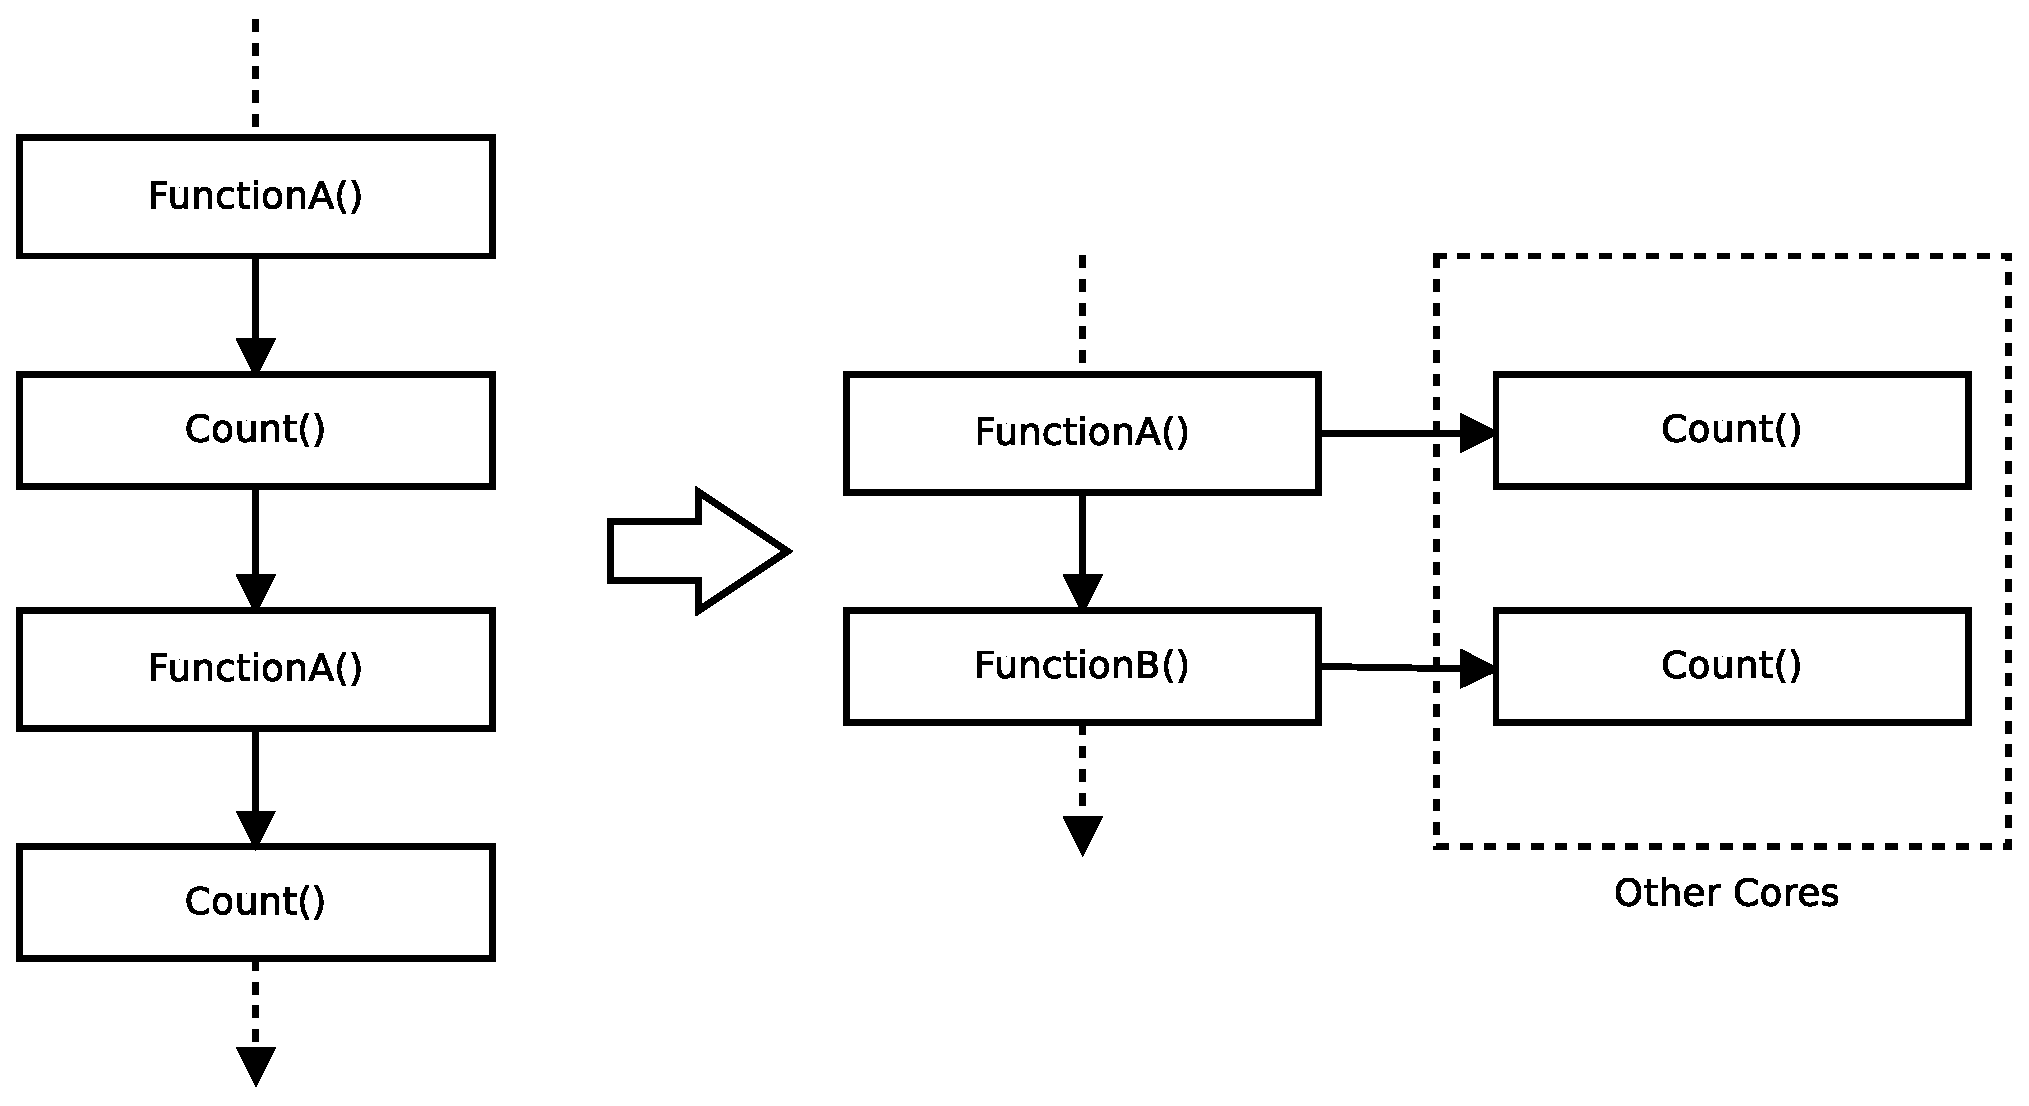
\includegraphics[width=0.8\textwidth]{chap1/Dig1}
  \bicaption[fig:dig1]{函数计数的简单例子}{函数计数的简单例子}{Table}{A simple example of method count}
\end{figure}

与此类似,很多其他的分析程序也可以进行并行化的处理。文献\cite{paSpeed}中指出,在串行执行的情况下,二进制动态程序分析可能会导致高达1000倍缓慢的速度。这是会很大程度上影响到被分析程序本身的。因此,将分析程序与被分析程序分离开来执行,理论上能提升动态分析的效率。

\section{已有解决方案}

Shadow profiling\cite{shaPro}是采用并行化进行程序分析的一个方案。不同于以往串行执行中直接一起执行分析程序与被分析程序,它创建了一个处理的线程,称为影子线程,专门用于处理和执行分析程序。由于利用了现代操作系统里基于拷贝的创建子进程操作,Shadow profiling中的处理线程可以认为是父线程(即被分析程序)的一个拷贝。但由于采用这种方式,各个线程之间是共享地址空间的,故而在程序安全方面不能得到保证。

Superpin\cite{superPin}则是另一个比较有名的动态并行程序分析框架,它采用了Pin作为动态注入的工具,在此基础上进行并行化的处理。与Shadow profiling不同的是,Superpin是将被分析程序以时间片为单位进行切分,通过对这些时间片以拷贝进程的方式进行并行,从而达到提高效率的效果。由于父线程即被分析程序没有引入很多的负载,所以可以全速运行,而子进程则相应地执行相关的并行任务。每个时间片都有相应的开始信号和停止信号,用以完成CPU之间的同步和任务的交付。这个框架主要有几个方面的问题需要考虑:

\begin{itemize}
	\item 任务之间的时序和同步。各个任务在原程序中是以一定的时序执行的,如何保证在并行执行的过程中这些任务仍以一定的顺序执行而不产生同步问题或者结果出错是一个问题。
	\item 系统调用的问题。父线程和子线程中对系统调用的处理必须保持一致性。
	\item 超时问题。由于采用了多线程和时间切片的方式,所以时序同步十分重要,应该正确处理好超时等情况。
	\item 侦测签名/时间戳的问题。该系统采用了一个唯一的签名作为一个时间切片开始的标志,从而使得系统状态得以被描述,从而使得时间切片间不会出现不合理的重叠,从而打乱执行顺序。
	\item 结果合并。并行的结果分别由不同的线程得出,此时各个线程的结果需要进行合并。
\end{itemize}

Trident\cite{eventDri}与前两者相比,采用了硬件支持的解决方案。通过采用事件驱动,它能有效地发现程序运行时所存在的优化的可能性,然后使用空闲线程对原程序进行动态优化,从而有效地提高整个程序的效率。硬件辅助的引入,使得这个发现的过程更加高效,减少了对主线程的开销。但相比于前两者,该工具只是进行了并行的动态优化,实质上整个原程序仍然是没有并行执行的。

\section{本文的解决方案}

在以往的解决方案中,并行进行程序分析的主要思想在于将对被分析程序没有影响的一些分析任务与被分析程序分离开来,使用空闲的线程和计算资源进行并行处理。但是该分离过程需要参数传递,线程创建,函数调用等过程。如果是细颗粒的一些任务,在并行处理的过程中,调用的次数会相对频繁很多,造成的结果就是多次调用造成的开销变多。

例如在Java中,如果我们以方法为单位进行并行分析,意即一个方法是一个分析任务,每次遇到分析点的时候即调用相关的方法进行处理,此时主线程即被分析程序就可以继续执行下去,分析程序被交付给其他的处理线程进行处理,从而能提高程序分析的效率。理论上这个方法是可行而且高效的,但在实际应用中,线程间的通信,沟通和同步所花费的开销就要大很多了。

还是以之前的函数计数为例。例如我们需要计算整个Java程序执行的过程中一共执行了多少个方法,其中方法Count()被插桩在被分析程序的每个方法入口,一旦被调用,则往计数器执行加一的操作,直至程序运行结束,返回计数器值,就是执行的函数总数了。在这个例子中,未插桩之前的程序就是被分析程序,而Count()方法就是分析程序。如果被分析程序是个比较庞大的程序,那么Count()方法就会被调用很多次,可能是几千甚至上万次。在这个情况下如果我们采用简单的并行的方法,那么整个完成并行的过程就需要相应次数的参数传递、进程间通信等过程;另一方面,由于Count()本身是完成对计数器加一的操作,因而是一个比较轻量级的操作,每次执行的开销并不算大。这两个因素造成的一个结果就是并行处理之后的程序在效率上有的时候并没有比原程序高,相反反而降低了。

为了解决这种情况,本文的解决方案基于另一种新的解决方案,即基于缓存机制的程序并行化框架。需要被并行的方法并不会在执行的时候立即交付给并行线程进行处理,而是先缓存起来,等到累计到了一定的数量的时候,才一起交付。在这种情况下,本来需要进行多次的进程间通信被缩减为一次,从而降低了在构建并行线程的时候的开销。在该方案的基础上,本文对其进行了一些相关的优化。

\section{本章小结}

本章阐述了程序分析技术的进步,并指出了一些程序分析技术在效率上的不足,并提出了通过并行化来解决这一问题的一个方案。接下来介绍了几个比较有名的工具和框架,并比较了他们在并行化处理程序分析上的一些异同。最后本文阐述了以往并行框架存在的一些缺点,并提出了相应的解决方案。

% PiPA\cite{pipa}是一种现有的并行化程序分析的方案,它采用了DynamoRIO作为二进制动态代码插桩工具来生成并行代码

%%==================================================
%% chapter02.tex for SJTU Master Thesis
%% based on CASthesis
%% modified by wei.jianwen@gmail.com
%% Encoding: UTF-8
%%==================================================

\chapter{一些 \LaTeX 排版的例子}
\label{chap:example}

\section{数学排版的例子}
\label{sec:matheq}

\subsection{公式排版}
\label{sec:eqformat}

这里有举一个长公式排版的例子,来自\href{http://www.tex.ac.uk/tex-archive/info/math/voss/mathmode/Mathmode.pdf}{《Math mode》}:

\begin {multline}
  \frac {1}{2}\Delta (f_{ij}f^{ij})=
  2\left (\sum _{i<j}\chi _{ij}(\sigma _{i}-
    \sigma _{j}) ^{2}+ f^{ij}\nabla _{j}\nabla _{i}(\Delta f)+\right .\\
  \left .+\nabla _{k}f_{ij}\nabla ^{k}f^{ij}+
    f^{ij}f^{k}\left [2\nabla _{i}R_{jk}-
      \nabla _{k}R_{ij}\right ]\vphantom {\sum _{i<j}}\right )
\end{multline}

\subsubsection{一个四级标题}
\label{sec:depth4}

这是全文唯一的一个四级标题。在这部分中将演示可伸长符号(箭头、等号的例子)的例子,以及如何在可伸长的符号上标注。在\href{http://zhou63.ahut.edu.cn/latex/ctexfaq.pdf}{《CTeX常见问题集》}中也由类似的介绍。
首先需要在diss.tex导言区引入如下的内容:

\begin{lstlisting}[language={TeX}, caption={插入导言区的内容}]
  \makeatletter
  \def\ExtendSymbol#1#2#3#4#5{\ext@arrow 0099{\arrowfill@#1#2#3}{#4}{#5}}
  \def\RightExtendSymbol#1#2#3#4#5{\ext@arrow 0359{\arrowfill@#1#2#3}{#4}{#5}}
  \def\LeftExtendSymbol#1#2#3#4#5{\ext@arrow 6095{\arrowfill@#1#2#3}{#4}{#5}}
  \makeatother
  
  \newcommand\myRightarrow[2][]{\RightExtendSymbol{=}{=}{\Rightarrow}{#1}{#2}}
  \newcommand\myLeftarrow[2][]{\LeftExtendSymbol{\Leftarrow}{=}{=}{#1}{#2}}
  \newcommand\myBioarrow[2][]{\ExtendSymbol{\Leftarrow}{=}{\Rightarrow}{#1}{#2}}
  \newcommand\myLongEqual[2][]{\ExtendSymbol{=}{=}{=}{#1}{#2}}
\end{lstlisting}

然后,在正文插入如代码\ref{mathextend}所示的内容。效果如下:

\begin{lstlisting}[language={TeX}, caption={可伸长的符号},label=mathextend,float]
  \begin{eqnarray}
    f(x) & \myBioarrow{A=B}  & B \\
    & \myLongEqual{A=B} & B \\
    & \myLeftarrow[A=B^2]{B=A^2} & B \nonumber \\
    & \myRightarrow{B^2=A^2} & B
  \end{eqnarray}
\end{lstlisting}

\begin{displaymath}
    A \xleftarrow{n=0} B \xrightarrow[LongLongLongLong]{n>0} C 
\end{displaymath}

\begin{eqnarray}
  f(x) & \myBioarrow{A=B}  & B \\
  & \myLongEqual{A=B} & B \\
  & \myLeftarrow[A=B^2]{B=A^2} & B \nonumber \\
  & \myRightarrow{B^2=A^2} & B
\end{eqnarray}

又如:

\begin{align}
  \label{eq:none}
  & I(X_3;X_4)-I(X_3;X_4|X_1)-I(X_3;X_4|X_2) \nonumber \\
  \myLongEqual{a)}\, & [I(X_3;X_4)-I(X_3;X_4|X_1)]-I(X_3;X_4|\tilde{X}_2) \\
  \myLongEqual[\rule{0.28cm}{0cm}]{}\, & I(X_1;X_3;X_4)-I(X_3;X_4|\tilde{X}_2)
\end{align}


\subsection{定理环境}

模板中定义了丰富的定理环境
algo(算法),thm(定理),lem(引理),prop(命题),cor(推论),defn(定义),conj(猜想),exmp(例),rem(注),case(情形),
bthm(断言定理),blem(断言引理),bprop(断言命题),bcor(断言推论)。
amsmath还提供了一个proof(证明)的环境。
这里举一个``定理''和``证明''的例子。
\begin{thm}[留数定理]
\label{thm:res}
  假设$U$是复平面上的一个单连通开子集,$a_1,\ldots,a_n$是复平面上有限个点,$f$是定义在$U\backslash \{a_1,\ldots,a_n\}$上的全纯函数,
  如果$\gamma$是一条把$a_1,\ldots,a_n$包围起来的可求长曲线,但不经过任何一个$a_k$,并且其起点与终点重合,那么:

  \begin{equation}
    \label{eq:res}
    \ointop_{\gamma}f(z)\,\mathrm{d}z = 2\uppi\mathbf{i}\sum^n_{k=1}\mathrm{I}(\gamma,a_k)\mathrm{Res}(f,a_k)
  \end{equation}

  如果$\gamma$是若尔当曲线,那么$\mathrm{I}(\gamma, a_k)=1$,因此:

  \begin{equation}
    \label{eq:resthm}
    \ointop_{\gamma}f(z)\,\mathrm{d}z = 2\uppi\mathbf{i}\sum^n_{k=1}\mathrm{Res}(f,a_k)
  \end{equation}

      % \oint_\gamma f(z)\, dz = 2\pi i \sum_{k=1}^n \mathrm{Res}(f, a_k ). 

  在这里,$\mathrm{Res}(f, a_k)$表示$f$在点$a_k$的留数,$\mathrm{I}(\gamma,a_k)$表示$\gamma$关于点$a_k$的卷绕数。
  卷绕数是一个整数,它描述了曲线$\gamma$绕过点$a_k$的次数。如果$\gamma$依逆时针方向绕着$a_k$移动,卷绕数就是一个正数,
  如果$\gamma$根本不绕过$a_k$,卷绕数就是零。

  定理\ref{thm:res}的证明。
  
  \begin{proof}
    首先,由……

    其次,……

    所以……
  \end{proof}
\end{thm}

上面的公式例子中,有一些细节希望大家注意。微分号d应该使用``直立体'',也就是用mathrm包围起来。
并且,微分号和被积函数之间应该有一段小间隔,可以插入\verb+\,+得到。
斜体的$d$通常只作为一般变量。
i,j作为虚数单位时,也应该使用``直立体'',为了明显,还加上了粗体,例如\verb+\mathbf{i}+。斜体$i,j$通常用作表示``序号''。
其他字母在表示常量时,也推荐使用``直立体'',譬如,圆周率$\uppi$(需要upgreek宏包),自然对数的底$\mathrm{e}$。
不过,我个人觉得斜体的$e$和$\pi$很潇洒,在不至于引起混淆的情况下,我也用这两个字母的斜体表示对应的常量。


\section{向文档中插入图像}
\label{sec:insertimage}

\subsection{支持的图片格式}
\label{sec:imageformat}

\XeTeX 可以很方便地插入PDF、EPS、PNG、JPG格式的图片。

插入PNG/JPG的例子如\ref{fig:SRR}所示。
这两个水平并列放置的图共享一个``图标题''(table caption),没有各自的小标题。

\begin{figure}[!htp]
  \centering
  
\includegraphics[width=0.3\textwidth]{chap2/testpng}
  \hspace{1cm}
  
\includegraphics[width=0.3\textwidth]{chap2/testjpg}
  \bicaption[fig:SRR]{这里将出现在插图索引中}{中文题图}{Fig}{English caption}
\end{figure}

这里还有插入eps图像和pdf图像的例子,如图\ref{fig:pdfeps}。这里将EPS和PDF图片作为子图插入,每个子图有自己的小标题。并列子图的功能是使用subfigure宏包提供的。

\begin{figure}
  \centering
  \subfigure[EPS Figure]{
    \label{fig:epspdf:a} %% label for first subfigure
    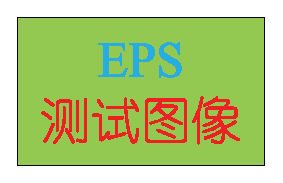
\includegraphics[width=0.3\textwidth]{chap2/testeps}}
  \hspace{1in}
  \subfigure[PDF Figure]{
    \label{fig:epspdf:b} %% label for second subfigure
    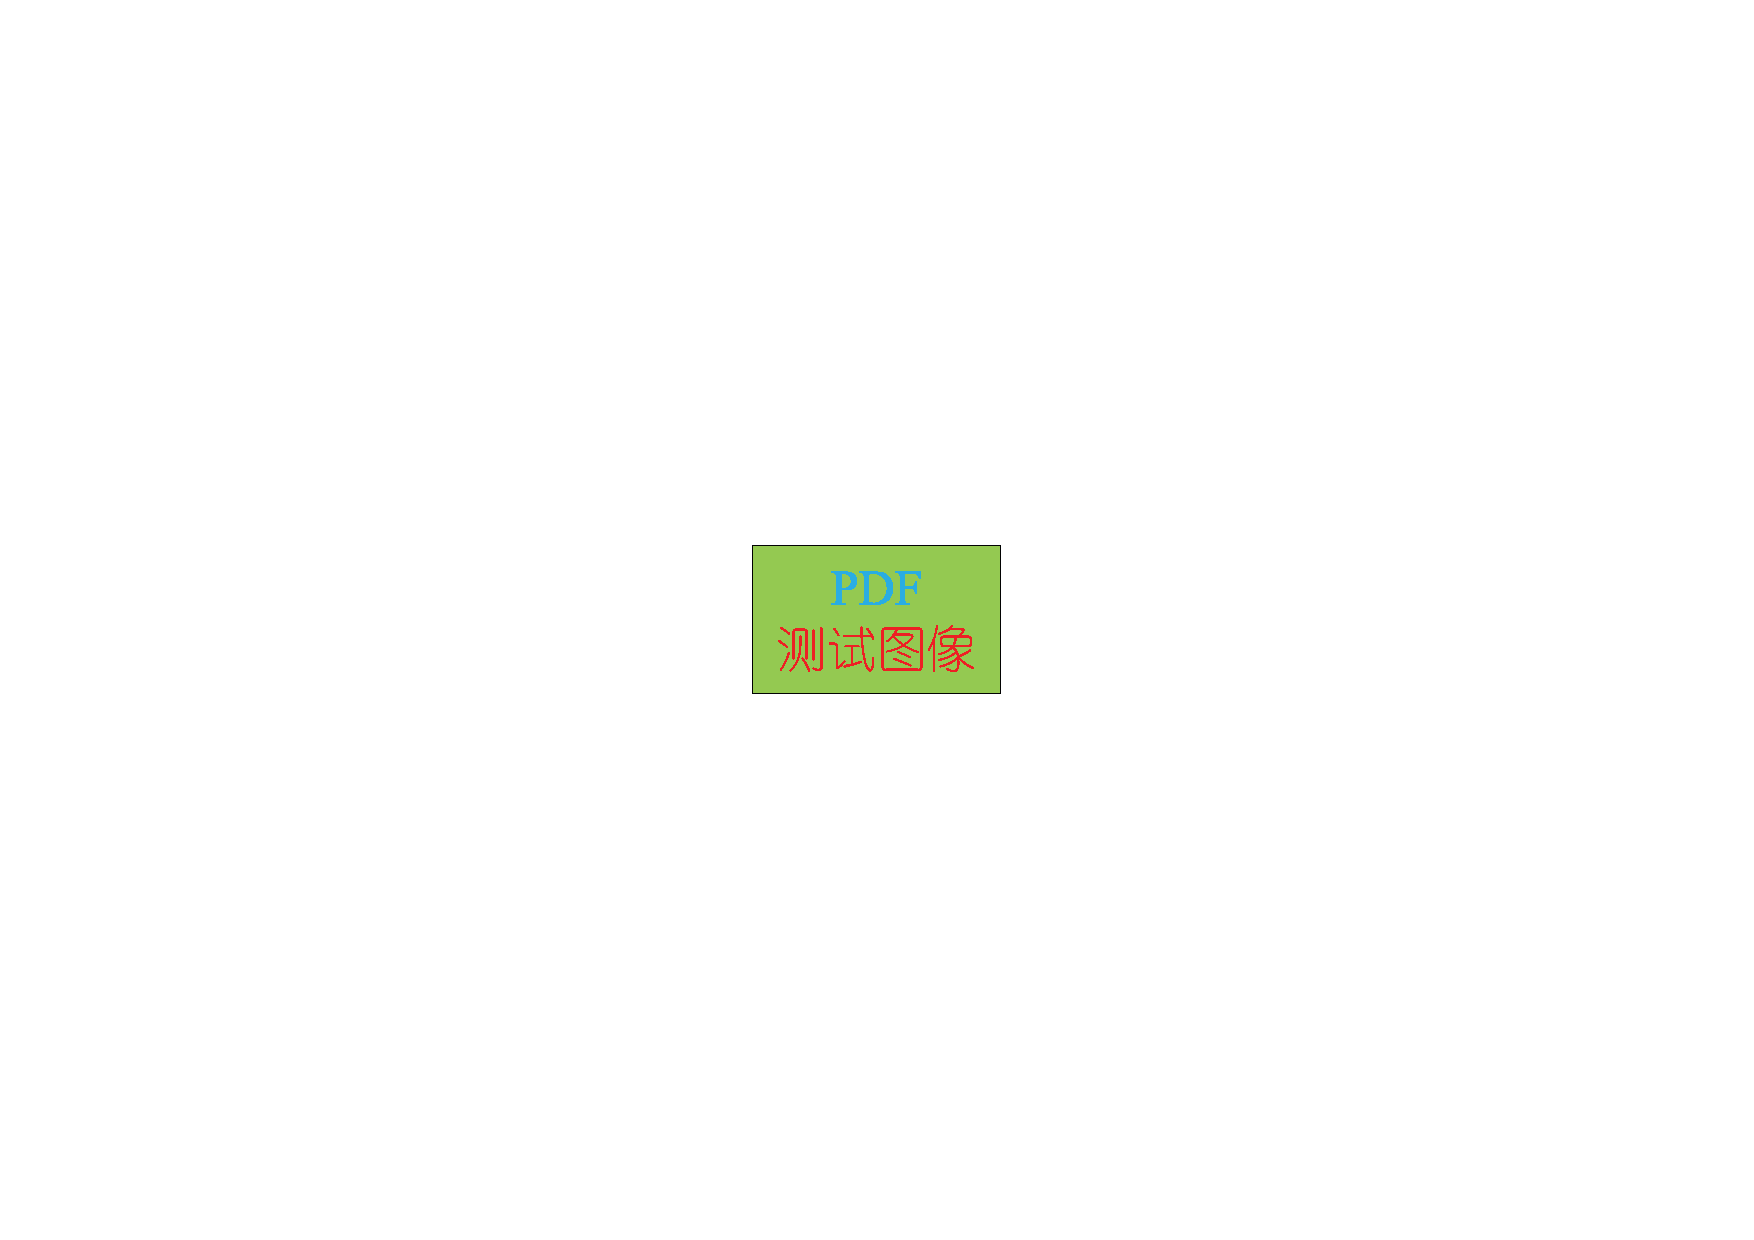
\includegraphics[angle=-90,origin=br,width=0.3\textwidth]{chap2/testpdf.pdf}}
  \bicaption[fig:pdfeps]{插入eps图像和pdf图像}{插入eps和pdf的例子}{Fig}{An EPS and PDF demo}
\end{figure}

更多关于 \LaTeX 插图的例子可以参考\href{http://www.cs.duke.edu/junhu/Graphics3.pdf}{《\LaTeX 插图指南》}。

\subsection{长标题的换行}
\label{sec:longcaption}

图\ref{fig:longcaptionbad}和图\ref{fig:longcaptiongood}都有比较长图标题,通过对比发现,图\ref{fig:longcaptiongood}的换行效果更好一些。
其中使用了minipage环境来限制整个浮动题的宽度。

\begin{figure}[!htp]
 \centering
 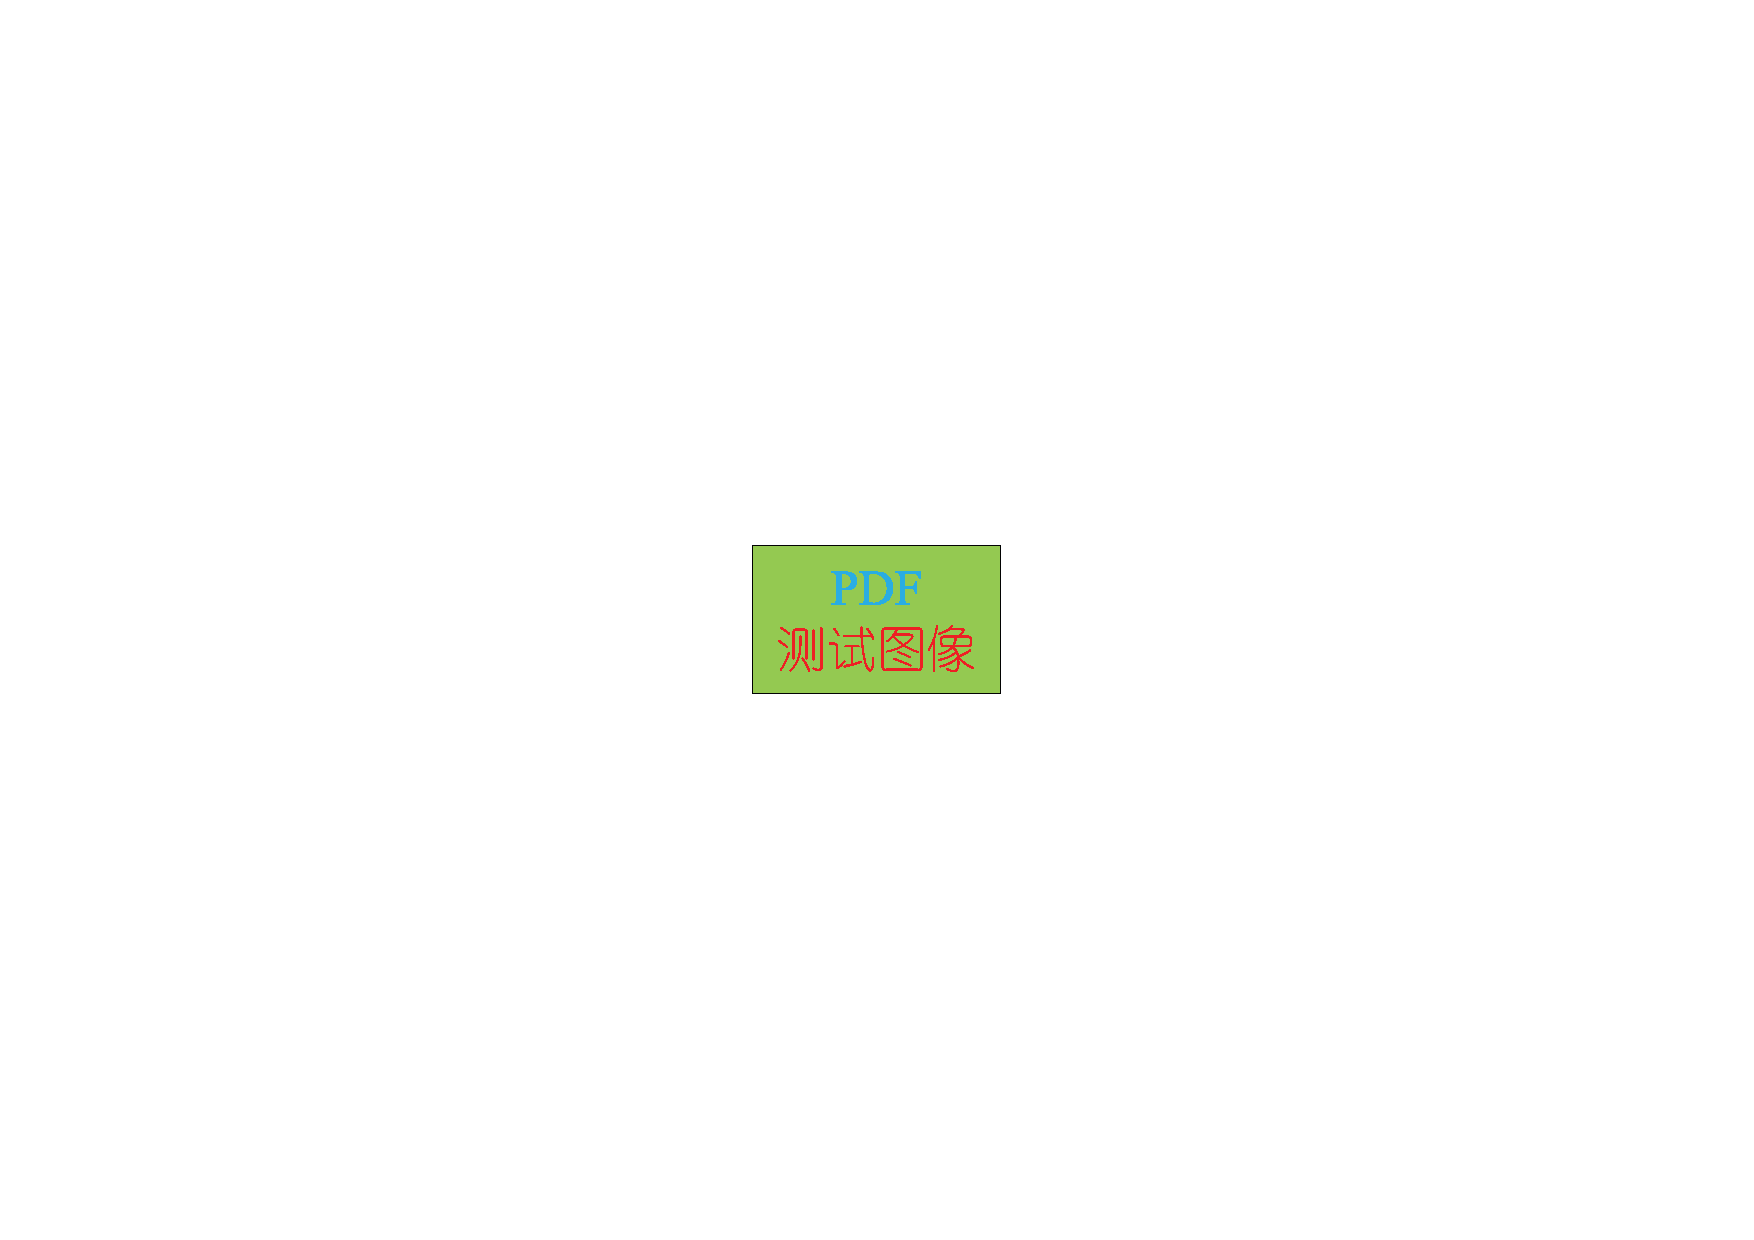
\includegraphics[angle=-90,origin=br,width=4cm]{chap2/testpdf.pdf}
 \bicaption[fig:longcaptionbad]{这里将出现在插图索引}{海交通大学是我国历史最悠久的高等学府之一,是教育部直属、教育部与上海市共建的全国重点大学.}{Fig}{Where there is a will, there is a way.}
\end{figure}


  \begin{figure}[!hbp]
    \centering
    \begin{minipage}[b]{0.6\textwidth}
      \captionstyle{\centering}
      \centering
      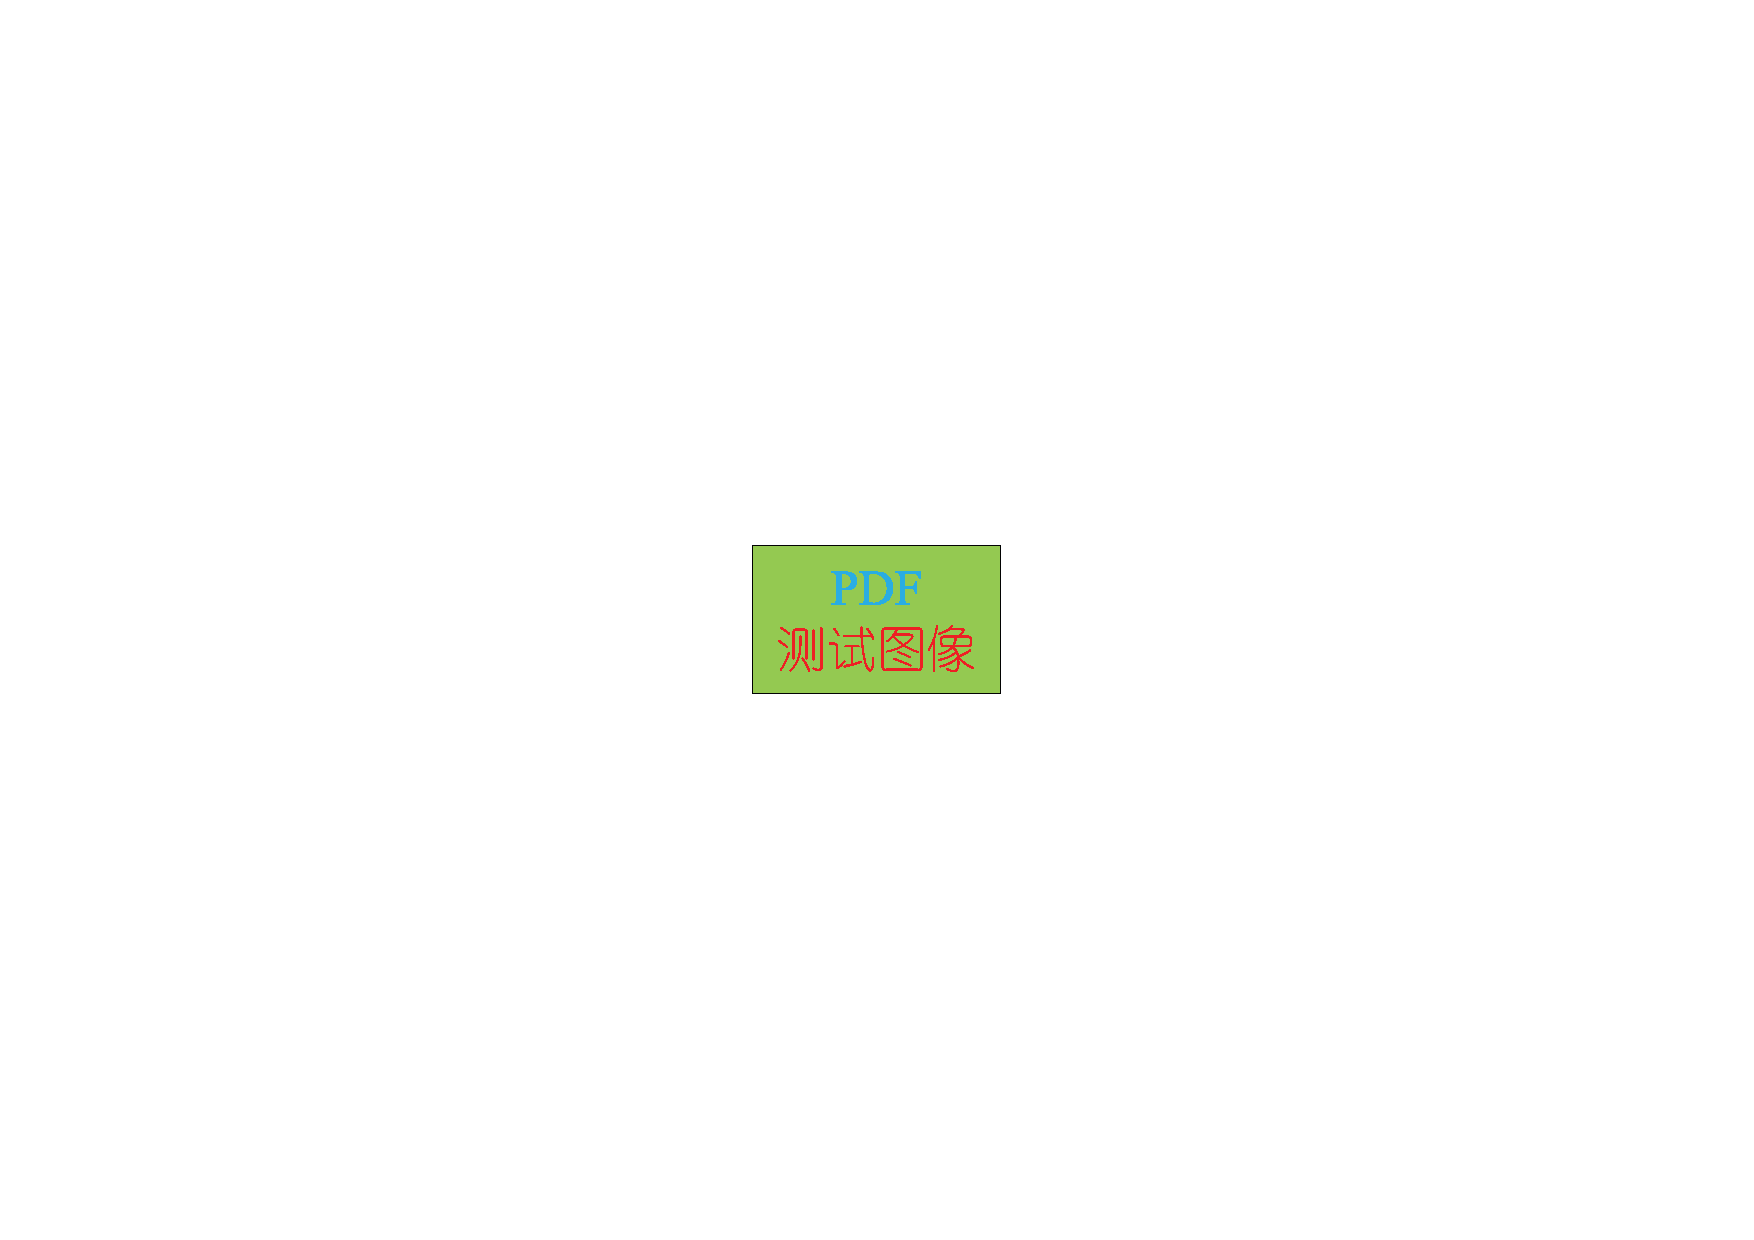
\includegraphics[angle=-90,origin=br,width=4cm]{chap2/testpdf.pdf}
      \bicaption[fig:longcaptiongood]{这里将出现在插图索引}{海交通大学是我国历史最悠久的高等学府之一,是教育部直属、教育部与上海市共建的全国重点大学.}{Fig}{Where there is a will, there is a way.}
    \end{minipage}     
  \end{figure}

  
\section{表格的例子}
\label{sec:tab}

这一节给出的是一些表格的例子,如表\ref{tab:firstone}所示。

\begin{table}[!hpb]
  \centering
  \bicaption[tab:firstone]{指向一个表格的表目录索引}{一个颇为标准的三线表格\footnotemark[1]}{Table}{A Table}
  \begin{tabular}{@{}llr@{}} \toprule
    \multicolumn{2}{c}{Item} \\ \cmidrule(r){1-2}
    Animal & Description & Price (\$)\\ \midrule
    Gnat & per gram & 13.65 \\
    & each & 0.01 \\
    Gnu & stuffed & 92.50 \\
    Emu & stuffed & 33.33 \\
    Armadillo & frozen & 8.99 \\ \bottomrule
  \end{tabular}
\end{table}
\footnotetext[1]{这个例子来自\href{http://www.ctan.org/tex-archive/macros/latex/contrib/booktabs/booktabs.pdf}{《Publication quality tables in LATEX》}(booktabs宏包的文档)。这也是一个在表格中使用脚注的例子,请留意与threeparttable实现的效果有何不同。}

下面一个是一个更复杂的表格,用threeparttable实现带有脚注的表格,如表\ref{tab:footnote}。

\begin{table}[!htpb]
  \bicaption[tab:footnote]{出现在表目录的标题}{一个带有脚注的表格的例子}{Table}{A Table with footnotes}
  \centering
  \begin{threeparttable}[b]
     \begin{tabular}{ccd{4}cccc}
      \toprule
      \multirow{2}{6mm}{total}&\multicolumn{2}{c}{20\tnote{1}} & \multicolumn{2}{c}{40} &  \multicolumn{2}{c}{60}\\
      \cmidrule(lr){2-3}\cmidrule(lr){4-5}\cmidrule(lr){6-7}
      &www & k & www & k & www & k \\
      \midrule
      &$\underset{(2.12)}{4.22}$ & 120.0140\tnote{2} & 333.15 & 0.0411 & 444.99 & 0.1387 \\
      &168.6123 & 10.86 & 255.37 & 0.0353 & 376.14 & 0.1058 \\
      &6.761    & 0.007 & 235.37 & 0.0267 & 348.66 & 0.1010 \\
      \bottomrule
    \end{tabular}
    \begin{tablenotes}
    \item [1] the first note.% or \item [a]
    \item [2] the second note.% or \item [b]
    \end{tablenotes}
  \end{threeparttable}
\end{table}

\section{参考文献管理}

参考文献的管理是这个学位论文模板又一个好玩的地方。

\subsection{将参考文献的内容与表现分离}

这个论文模板使用BibTeX处理参考文献,这又是一个``内容''与``表现形式''分离的极好例子
\footnote{当然,你也可以手动编参考文献item,直接插入文档中。但是,有BibTeX帮助,我觉得没有人想用这种麻烦的方法,所以就在脚注中说明了。}。
参考文献的``内容''就是reference文件夹下的chap\textit{xx}.bib,参考文献的元数据(名称、作者、出处等)以一定的格式保存在这些纯文本文件中。
.bib文件也可以理解为参考文献的``数据库'',正文中所有引用的参考文件条目都会从这些文件中``析出''。
控制参考文献条目``表现形式''(格式)的是.bst文件。.bst文件定义了参考文献风格,使用不同的参考文献风格能将同一个参考文献条目输出成不同的格式。
当然,一个文档只能使用一个参考文献风格。
按照教务处的要求,本模板使用的是国标GBT7714风格的参考文献。

BibTeX的工作过程是这样的:
BibTeX读取.aux(第一次运行latex得到的)看看你引用了什么参考文献条目,
然后到.bib中找相关条目的信息,
最后根据.bst的格式要求将参考文献条目格式化输出,写到.bbl文件中。
在运行latex将.bbl插入文档之前,你可以用文本编辑器打开它,做一些小的修改。
你会发现,.bbl的格式和你自己手动写item很相似,它已经被赋予了一定的``表现形式''。

.bib数据库中的参考文献条目可以手动编写,也可以在google的学术搜索中找到。
各大数据库\footnote{应该说是国际知名数据库,譬如SCOPUS, IEEE, OSA等,国内数据库在搜索、导出方面一直是差得一塌糊涂。}也支持将参考文献信息导出为.bib,
省时省力。
以Google学术搜索为例:进入\url{http://scholar.google.com},在``学术搜索设置''中,将``文献管理软件''设为``显示导入BibTeX''的连接,保存退出。
然后学术搜索找到文献下会有``导出到BibTeX''连接,点击后Firefox会打开新的标签页,出现类似代码\ref{googlescholar}所示的内容
\footnote{展示这些.bib条目使用了listings宏包,因为listings宏包协调中文的能力很糟糕,所以读者在查看模板的这部分源代码时会看到一些非常麻烦的东西。并且,直接将源代码的这部分内容复制到.bib中可能还会出错。我的建议是:这部分内容留意PDF就足够了。}。
请注意,这个条目离``规范''还有一些距离。

  \begin{lstlisting}[caption={从Google Scholar找到的,但并不规范的.bib条目}, label=googlescholar, float, escapeinside="", numbers=none]
    @phdthesis{"白2008信用风险传染模型和信用衍生品的定价",
      title={{"信用风险传染模型和信用衍生品的定价"}},
      author={"白云芬"},
      year={2008},
      school={"上海交通大学"}
    } 
  \end{lstlisting}

  上面的.bib条目的``名字''\cndash{}``白2008信用风险传染模型和信用衍生品的定价'',包含ASCII以外的字符,BibTeX无法处理;
  条目还缺少了address域,这样编译出来的结果会出现``地址不详'';
  并且,条目还缺少language域,BibTeX需要language域来判断是否是中文参考文献。
  将上面的条目修正(改英文名、增加address和language域),复制到本地的.bib文件中就可以了。
  显然,这里描述的是参考文献的内容,而不是表现形式。

  \begin{lstlisting}[caption={一个符合规范的.bib条目}, label=itemok, float, escapeinside="", numbers=none]
    @phdthesis{bai2008,
      title={{"信用风险传染模型和信用衍生品的定价"}},
      author={"白云芬"},
      year={2008},
      language={zh},
      address={"上海"},
      school={"上海交通大学"}
    } 
  \end{lstlisting}

由于中英文参考文献处理起来有差异,所以需要在参考文献中标注是否是中文文献。
确切地说,BibTeX并不具有区分中英文参考文献的``智能'',这种智慧的来源是.bst文——它定义了处理参考文献的规则。
GBT7714-2005NLang.bst中规定:.bib中的条目,如果条目的``language''域非空,就被认为是中文文献,否则被认为是英文文献。
例如,刚才的文献,就会被认为是中文参考文献,采取一些针对中文的处理方式。

最后,这个条目被bibtex处理后,赋予了一定的``表现形式'',在.bbl文件中以下面的样子出现。
你还可以对它进行小的修改,这是一种很折磨人的终极修改方法。
再次运行latex之后,它将被插入到文档中。

\begin{lstlisting}[caption={.bbl中被格式化之后的条目}, escapeinside="", numbers=none]
\bibitem["白云芬(2008)"]{bai2008}
  \textsc{"白云芬"}.
  \newblock {"信用风险传染模型和信用衍生品的定价"}[D].
  \newblock "上海: 上海交通大学, 2008."
\end{lstlisting}

再罗嗦两句,
.bst文件书写起来非常繁杂\footnote{可以参考\href{http://ftp.ctex.org/mirrors/CTAN/info/bibtex/tamethebeast/ttb_en.pdf}{《Tame The BeaST》}。},书写符合GBT7714标准的.bst文件更是一项浩大的工程。
因此,当大家为漂亮、标准的参考文献列表感到满意时,应该对GBT7714-2005NLang.bst的作者充满谢意。
作者在CTeX BBS发的帖子,请看
\href{http://bbs.ctex.org/viewthread.php?tid=33571&highlight=\%B2\%CE\%BF\%BC\%CE\%C4\%CF\%D7\%2BGB}{文后参考文献著录规则 GB/T 7714-2005}。
关于GB/T 7714-2005标准本身,请看\href{http://bbs.ctex.org/viewthread.php?tid=33571&highlight=GB\%2B\%B2\%CE\%BF\%BC\%CE\%C4\%CF\%D7}{这里}。

再多说两句,.bib是“参考文献的内容”,而控制参考文献表现(格式)的是.bst文件,本模板附带的是GBT7714-2005NLang.bst。

\subsection{在正文中引用参考文献}

参考文献可以分章节管理,只需要在主文件中的参考文献中都包含进去就可以,如\verb+\bibliography{chap1,chap2,...}+。

正文中引用参考文献时,用\verb+\upcite{key1,key2,key3...}+可以产生“上标引用的参考文献”,
如\upcite{Meta_CN,chen2007act,DPMG}。
使用\verb+\cite{key1,key2,key3...}+则可以产生水平引用的参考文献,例如\cite{JohnD,zhubajie,IEEE-1363}。
请看下面的例子,将会穿插使用水平的和上标的参考文献:关于书的\cite{Meta_CN,JohnD,IEEE-1363},关于期刊的\upcite{chen2007act,chen2007ewi},
会议论文\cite{DPMG,kocher99,cnproceed},
硕士学位论文\cite{zhubajie,metamori2004},博士学位论文\upcite{shaheshang,FistSystem01,bai2008},标准文件\cite{IEEE-1363},技术报告\upcite{NPB2},电子文献\cite{xiaoyu2001, CHRISTINE1998},用户手册\cite{RManual}。

最后总结一些注意事项:
\begin{itemize}
\item 参考文献只有在正文中被引用了,才会在最后的参考文献列表中出现;
\item 参考文献``数据库文件''.bib是纯文本文件,请使用UTF-8编码,不要使用GBK编码;
\item 参考文献条目中通过language域是否为空判断是否是中文文献;
\item 参考文献条目同样有“内容”和“表现形式”之分,这种可控性是BibTeX带来的。
\end{itemize}


\subsection{参考文献管理器}

参考文献数据库.bib虽然是纯文本的,可以用任意的文本编辑器查看,但总有人喜欢一个找一个``可视化''地查看每一条参考文献。
我想\href{http://jabref.sourceforge.net/}{JabRef}应该是个很不错的选择。
这是一个Java写的程序,需要JRE才能运行。
就我测试的情况上看,很幸运,JabRef可以顺利打开GBK编码的.bib文件。
但是,打开UTF--8编码的.bib源文件过程中总会崩溃,原因不得而知。
由于我们的.bib文件使用的是UTF-8编码,所以JabRef暂时不可用。

提到参考文献管理器,不得不提到另一个广被使用的软件——\href{http://www.endnote.com/}{EndNote}。
在图书馆的宣讲会上,EndNote被吹得神乎其神,但我发现他对.bib的管理很不友好。
EndNote可以导入.bib文件,却不能导出.bib,只能导出.bbl——被格式化的.bib。
原来,JabRef比较``单纯'',不具备格式化参考文献的能力;
而EndNote有那么一点设置参考文献输出格式的能力,然后就把这种能力滥用,这点搞得我很不爽。
看来,EndNote和Word配合得更好一些。


\section{用listings插入源代码}

原先ctexbook文档类和listings宏包配合使用时,代码在换页时会出现莫名其妙的错误,后来经高人指点,顺利解决了。
感兴趣的话,可以看看\href{http://bbs.ctex.org/viewthread.php?tid=53451}{这里}。
这里给使用listings宏包插入源代码的例子,这里是一段C代码。
另外,listings宏包真可谓博大精深,可以实现各种复杂、漂亮的效果,想要进一步学习的同学,可以参考
\href{http://mirror.ctan.org/macros/latex/contrib/listings/listings.pdf}{listings宏包手册}。

\begin{lstlisting}[language={C}, caption={一段C源代码}]
#include <stdio.h>
#include <unistd.h>
#include <sys/types.h>
#include <sys/wait.h>

int main() {
  pid_t pid;

  switch ((pid = fork())) {
  case -1:
    printf("fork failed\n");
    break;
  case 0:
    /* child calls exec */
    execl("/bin/ls", "ls", "-l", (char*)0);
    printf("execl failed\n");
    break;
  default:
    /* parent uses wait to suspend execution until child finishes */
    wait((int*)0);
    printf("is completed\n");
    break;
  }

  return 0;
}
\end{lstlisting}

再给一个插入MATLAB代码的例子,感谢daisying站友提供的代码。

\begin{lstlisting}[language={matlab}, caption={一段MATLAB源代码}]
function paper1
r=0.05;
n=100;
T=1;
X=1;
v0=0.8;
sigma=sqrt(0.08);
deltat=T/n;
for i=1:n
    t(i)=i*deltat;
    w(i)=random('norm',0,t(i),1);
end
for i=1:n
    alpha(i)=0.39;
end
for i=1:n
    temp=0;
    for k=1:i
        temp=temp+alpha(k);
    end
    B(i)=exp(r*t(i));
    BB(i)=B(i)*exp(temp*deltat);
    BBB(i)=exp(-r*(T-t(i)));
end
for i=1:n
    s0(i)=X*BBB(i);
    v(i)=v0*exp((r-0.5*sigma^2)*t(i)+sigma*w(i));
    for j=i+1:n
        D=X*BBB(j);
        d1=(log(v(i)/D)+(r+sigma^2/2)*(t(j)-t(i)))/(sigma*sqrt(t(j)-t(i)));
        d2=d1-(sigma*sqrt(t(j)-t(i)));
        ppp(i,j)=D*exp(-r*(t(j)-t(i)))*(1-cdf('normal',d2,0,1))-v(i)*(1-cdf('n
ormal',d1,0,1));
    end
end
for i=1:n
    s1(i)=0;
    for j=i+1:n
        s1(i)=s1(i)+BB(j)^(-1)*alpha(j)*deltat*(X*BBB(j)-B(j)/B(i)*ppp(i,j));
    end
    s2(i)=0;
    for j=1:n
        s2(i)=s2(i)+alpha(j);
    end
    s2(i)=X*exp(-r*T-s2(i)*deltat);
    s(i)=BB(i)*(s1(i)+s2(i));
end
plot(s)
hold on;
plot(s0);
\end{lstlisting}

%%==================================================
%% chapter03.tex for SJTU Master Thesis
%% based on CASthesis
%% modified by wei.jianwen@gmail.com
%% Encoding: UTF-8
%%==================================================

\chapter{Deferred Method框架}

Deferred Method是瑞士卢加诺大学动态程序分析小组所开发的一套并行程序分析的框架。通过使用该框架,用户能够方便地在比较高层面进行编程,从而在不需要关心底层代码的执行状况的情况下,编写出高效的并行程序。该框架采用ASM作为动态代码生成的工具,效率较高。本章将通过概览、简单示例、设计框架、处理策略等几个方面对Deferred Method进行描述,并对其一些功能进行讨论。

\section{概览}

在一些其他的并行程序分析工具中,被分析程序的颗粒度较粗,多数情况下这些被并行的任务也是重量级的,同时具有可以乱序执行,不影响原程序等特点,所以这些并行程序能很好地完成多线程处理这些并行任务的功能,效率上也比较高。但当被并行的任务颗粒度较细的时候,执行任务本身的开销并不大,并行线程并没有得到很好的利用;另一方面,当这些任务被执行的次数较为频繁的时候,轻量级的任务被调用多次,耗费在进程间通信的开销有时甚至要大于单线程执行被分析程序的开销。

为了解决这一问题,学术界提出了一些解决的方法,其中一个代表性的方法就是前文提到的基于缓存机制的处理方法。基于这个方法开发的工具一般都会维护一个或多个缓存(例如为每个线程维护一个线程本地的缓存),每个缓存用于存储程序运行时遇到需要并行的任务的相关信息,例如被调用的函数名字或者id,调用参数等等。并行的时候,主线程并不会立即把参数传递给处理线程,而是先缓存起来,等到缓存满的时候,再一并交给处理线程进行处理。与原来的简单并行相比,这种方法能很有效地减少进程间通信,原来需要多次通信的调用现在被缩减为一次;另一方面,由于处理线程每次都能拿到整个缓存的调用,当缓存设置合适的时候,处理线程能够保持一段时间的高负载工作,从而提高了CPU的利用率。

Deferred Method框架即是基于这个思想进行开发和改进的。它能比较有效率地处理一些颗粒度比较小的任务,同时提供了一套可定制的处理线程的策略,例如同步执行,即缓存中的内容即交由主线程处理;例如线程池策略,即维护一定数量的线程和一个任务队列,空闲的线程从任务队列中取得任务进行处理。

Deferred Method提供了一套高层次的、易用性高的接口。它通过使用ASM作为工具,自动从用户定义好的Java类中分析取得相关的信息,并生成相应的代码。缓存任务,提交给处理线程等细节被隐藏起来,用户只需要关注高层的实现,而不需关心这些代码在字节码层面上的实现。这套接口同时也允许用户对诸如缓存大小、队列长度进行设置。与其他框架相比,这个框架引入了一些功能:

\begin{itemize}
	\item 多种处理策略。该框架提出了如单线程同步处理、线程池处理、自适应线程处理等多种策略。用户可根据CPU资源的利用情况自行选择需要使用的处理策略。例如在单核程序中,可以使用同步处理的方式、在多核处理中,可以采用线程池或自适应处理的策略。
	\item 结果合并。该框架提供了一个处理器钩子,用户能够使用这个钩子作为接口,定义在每个缓存执行前后所需要执行的一些代码;并为每个缓存提供了一个本地的变量池。用户利用这个机制,可以在缓存被处理前定义本地变量用于储存该次处理的结果,而后在处理完成后,将本地的结果合并到全局的结果中。采用该方法的优点是能减少对全局变量的访问,从而减少多线程同步所带来的开销,能有效地提高效率。
	\item 代码自动生成。相关的代码是由程序自动分析生成的,省去了用户对底层代码和注入过程的关注。
\end{itemize}

以下将通过一个简单的示例来演示Deferred Method的功能。

\section{简单示例}

以下是一段简单的函数计数的代码:

\begin{lstlisting}[language=Java]
public static void foo(){
	//注入的分析代码,即对计数器的调用
	methodCount();
	//原代码
	……
}
\end{lstlisting}

在该代码段中methodCount()是分析程序,用于方法计数。对该段程序进行并行化修改之后,对这个对方法进行计数的方法的执行过程就将交给处理线程进行处理。在Deferred Method中,由于采用的是缓存方法,程序将被改写为类似如下的代码:

\begin{lstlisting}[language=Java]
public static void foo(){
	//把对该方法的调用存储到缓存中
	if (getLocalBuffer().isFull){
		processCurrentBuffer();
		createBuffer();
	}
	addMethodCount();
	//原代码
	……
}
\end{lstlisting}

其中addMethodCount()方法是由Deferred Method框架自动分析生成的代码,用于将对methodCount()的调用信息进行记录和储存,以让处理线程能正确进行调用。修改后的代码在每次调用前先检查当前的缓存是否已满,如果满了的话,则将缓存先交付出去,给处理线程进行处理。整个代码的生成过程都是框架采用ASM作为字节吗修改工具进行生成的,用户只要在Java语言的层面上简单地做一些定义,即可完成这个编写并行分析程序的过程。

\section{框架结构}

本节介绍Deferred Method的框架结构,主要从框架的接口,用户定义类,框架自动生成的代码以及结果合并几个方面来阐述整个Deferred Method的框架的设计。

\subsection{框架接口}

Deferred Method的接口如图所示。

%\begin{figure}[!htp]
%\end{figure}[!htp]

其中,DeferredEnv集合了对整个Deferred Method框架的一些管理操作的方法,用户可以通过调用这些方法对这个框架和整个并行生成、执行过程进行监控和管理。其中,getBufferCapacity()方法可以得到缓存的大小。缓存的大小指的是该缓存能储存的最多的调用方法信息的数量,换言之,即在一般的执行中,缓存储存了多少方法后被系统视作为“满”的,从而交付给处理线程进行处理。如果这个数值没有进行初始化,Deferred Method默认会给它一个值。

相应地,setBufferCapacity(int)这个方法则是用于设置缓存的大小的方法。需要注意的是,调用该方法并不会影响当前正在使用的缓存的大小。只有当当前缓存用满被交予处理线程之后,系统自动创建一个新的缓存的时候,新建的线程才被设置为被修改后的缓存的大小。

processCurrentBuffer()方法则被用于将当前缓存交付予处理线程进行处理。在Deferred的默认框架中,当缓存变满时,它将会自动被交付,事实上即是调用了这个方法。Deferred Method框架将这个方法作为接口暴露给用户,主要是考虑到有些情况下用户希望能强制执行这个过程。

在类DeferredExecution中的方法createDeferredEnv(...)用于创建一个环境类,即前文所提到的DeferredEnv.通过传入特定的参数,这个类能够分析用户所定义的需要被并行执行的方法,然后动态生成需要的类和代码,最后返回一个DeferredEnv类的实例,以提供给用户接口进行操作。

\subsection{用户定义类}

还是以简单的函数计数作为例子,在Deferred Method中,用户如果需要将方法计数的方法methodCount()作为可以被并行的任务,需要先编辑两个类来定义它,相关代码如下:

\begin{lstlisting}[language=Java]
public interface Analyze extends Deferred{
	public void methodCount();
}

public class AnalyzeImpl implements Analyze{
	public void methodCount(){
		//把计数器加一的代码
		......
	}
}
\end{lstlisting}

该段代码定义了一个接口和一个实现类,其中实现类实现了该接口所定义的方法,在该例子中即是Analyze中的methodCount()方法。Analyze接口继承了Deferred Method内部库提供的一个Deferred类,以作为标志。在具体代码动态生成的时候,框架会检测Analyze是否继承了Deferred类。

用户定义好的接口和实现类在创建环境的时候,即调用createDeferredEnv(...)方法的时候,类本身会作为参数传递给该方法,该方法即分析这些类从而获得相关的需要并行的方法的信息。

\subsection{代码动态自动生成及调用}

在实际使用中,用户需要把定义的接口和类作为参数传递给创建环境的方法,然后在实际的使用中通过环境来调用需要被并行且已经定义在定义类中的方法。在本例中,相关代码如下:

\begin{lstlisting}[language=Java]
......
static final DeferredEnv<Analyze> def = 
		DeferredExecution.createDeferredEnv(Analyze.class, 
							AnalyzeImpl.class, 
							new ThreadPoolProc());
static final Analyze mc = def.getProxy();
......

public void foo(){
	mc.methodCount();
	//原代码
	.....
}
\end{lstlisting}

在该段代码中为了能使用程序并行化,首先需要创建一个DeferredEnv的环境。之前所定义的接口Analyze和对于该接口的实现AnalyzeImpl被作为参数传递给创建环境的方法。该方法接受了这两个参数后,首先开始检查这个接口是否继承了Deferred类,继而对该接口进行分析,对各个方法进行标志,分析它们的调用参数,以便之后进行处理。

接着,这个创建方法开始创建相关的类。首先它会根据缓存大小的设置和用户定义类创建一个缓存类GeneratedBuffer,它包含了一些列的数组,用于记录函数调用的信息,如调用函数的ID,调用参数等。然后方法以用户自定义类的实现(在本例中是AnalyzeImpl)为基础,开始重写一个DeferredEnv类。该类将AnalyzeImpl中的方法的行为都改写成将该方法的ID存储到相应的缓存中,并使用相同的名字,以便用户使用的时候方便调用。而真正相应的方法被隐藏起来,只有处理线程在处理的时候根据ID才能进行调用。

经过代码处理后的类具有与AnalyzeImpl相同的方法,但方法行为已经改变,用户在实际调用这些方法的时候,事实上是调用了“把这些函数的调用信息暂时储存在缓存中”的方法。在完成了这一过程后,框架还在该环境中加入前文所说的一些方法,例如获得缓存大小的getBufferCapacity(),处理当前缓存的processCurrentBuffer()等。

当缓存满了的时候,它会被送至处理线程处进行处理。处理线程是一系列实现了一定接口的类,它们的区别在于不同的多线程处理策略。缓存单元,即GeneratedBuffer类本身实现了Runable接口,而接口所带的run()方法即是根据记录在该缓存中的信息调用相关方法的过程。

除了以上的基本功能之外,Deferred Method框架还支持结果合并的功能,这也是它区别于其他很多框架的一个功能。由于有些分析程序的结果需要储存在全局的变量中,例如内容调用树、方法调用的计数器等。由于整个并行的过程中都对这些变量进行访问,所以会有同步的问题需要考虑。如果不使用同步机制,那么对这些共享变量的访问将导致数据写入的错误,影响结果;而另一方面,如果引入锁等机制,将会不可避免地造成阻塞,影响了并行执行的效率,从而与并行框架的初衷和目的相违背。

Deferred Method引入了本地结果与全局结果相合并的方法来处理这个问题。它提供了ProcessingHook这个接口,使得用户可以通过这个接口来定义并行程序在处理每个缓存时所应当具有的行为。

还是以方法计数为例,这个接口的使用方法如下:

\begin{lstlisting}[language=Java]

public interface Analyze extends Deferred{
	public void methodCount();
}

public class AnalyzeImpl implemenots Analyze, ProcessingHooks{
	static final AtomicInteger global = new AtomicInteger();
	private int local;

	public beforeProcessing(){
		local = 0;
	}

	public void methodCount(){
		//把本地计数器加一的代码
		local++;
		......
	}

	public void afterProcessing(){
		global.addAndGet(local);
	}
}
\end{lstlisting}

在该例子中,引入了ProcessingHooks这个接口,实现该接口的类必须具有beforeProcessing()和afterProcessing()这两个方法。beforeProcessing()方法主要用于设置程序在处理缓存前的行为,而afterProcessing()方法主要用于设置程序在处理缓存后的行为。

该实现类定义了一个全局公有的变量为global,这是一个支持原子操作的变量,以保证该变量的原子性。任何两个以上的线程如果不能同时访问这个变量,以保证数据的正确性。当一个线程在访问和修改该变量的时候,如果有其他的线程也需要访问和修改,则必须阻塞等待,知道该线程访问完成。

而本地变量则为每个GeneratedBuffer类实例所私有,作为一个局部的结果,等到处理完成后再合并到全局的结果中。在这个例子里,局部变量为local,每次调用methodCount()方法的时候,实质上是往local本地变量上执行加一的操作。由于这个变量是GeneratedBuffer的每个实例所私有与维护,所以不会产生同步的问题。

在执行createDeferredExecution(...)方法的时候,该方法会读取AnalyzeImpl类中所实现的接口,如果这些接口中含有ProcessingHooks接口,方法会在返回的DeferredEnv环境和生成的GeneratedBuffer类中加入相关的信息。处理线程在处理这些信息的时候,由于调用了run()方法,而run()方法已经被改写加入了调用beforeProcessing()和afterProcessing()的方法,所以能成功地在处理缓存开始前与结束后分别对局部结果做初始化以及合并到全局结果的工作。

\section{缓存的处理策略}

Deferred Method提供了多种处理策略,如同步的处理策略,基于线程池的异步处理策略,以及自适应的处理策略等。以下将详述几种处理策略。

\subsection{同步处理策略}

同步处理策略,简单地将,即是由主线程同时执行缓存中的任务,即在这个模型里,只有生产者,没有消费者。故而这个模型严格地说并不是一个并行执行的程序模型,它所执行的内容是伪并行的。

它在实现上的一个基本的原理是在缓存满的时候,框架会执行processCurrentBuffer()方法,该方法能把当前缓存交付给处理线程执行,而在同步的处理策略中,这个交付的过程事实上就是直接执行GeneratedBuffer的Run()方法,即处理当前缓存。

与其他不采用缓存和并行的串行执行的程序分析相比,同步的处理策略事实上还引入了一些额外的开销,例如缓存的分配、初始化,DeferredEnv环境的生成等等。但在采用结果合并功能的实现中,由于采用了本地化的方法,一些被分析程序也存在着通过这个策略优化的空间。

例如在本身是多线程的程序中,如果整个程序也维持着一些全局的变量,那么被分析程序在多线程中执行,也有可能会频繁访问这些变量,造成效率的低下。这个时候如果使用同步处理策略的模型,则可以使用结果合并的思想,先以缓存为单位将这些变量在局部进行处理,处理完成后再合并到全局的变量中。通过这种方式,原本对共享数据段的多次访问变成了一次访问,从而能有效地提高

%%==================================================
%% chapter03.tex for SJTU Master Thesis
%% based on CASthesis
%% modified by wei.jianwen@gmail.com
%% Encoding: UTF-8
%%==================================================

\chapter{Java并行框架的功能优化实现}

前文介绍了Deferred Method并行框架。该框架提供了一套易用性高的接口给用户,允许用户在高层次上实现一套自己的代码注入方案。但该方案事实上仍存在着一些不足,例如:

\begin{itemize}
	\item 时序的问题。由于同步处理的方法是单线程执行,故而时序上是可以得到保证的,但这种方法并不是严格并行的;采用基于线程池的异步处理策略和自适应的策略保证了多线程的并行性,但在时序上会产生问题。
	\item 处理策略的问题。该框架只提供了三种策略,这三个策略只是给予用户通过简单地从可用核心的数量上来区分和决定需要使用的策略的选择的,而没有其他的处理策略能通过其他的情况来考虑,例如通过原程序的线程使用情况。
	\item 提交缓存的问题。该框架只有在缓存满的情况下才会自动提交缓存,但事实上有的时候会出现一些情况,使得缓存长时间无法被填满,此时缓存中所储存的方法无法被及时地处理,浪费了空闲的计算资源。
	\item 返回值的问题。该框架只能处理没有返回值的方法,有些分析程序需要在特定的时候使用到之前的分析程序的分析结果,这在Deferred Method默认提供的接口里是无法实现的。
\end{itemize}
		
本章将针对这些问题,一一进行阐述,并提出解决方案和设计。

\section{时序问题和检查点(CheckPoint)的使用}

\subsection{概述}

在前文所列举的方法计数的例子中,由于计数器对原程序的执行并没有时序要求,所以分析程序可以乱序执行;但在一些程序分析的例子里,却存在着时序的约束。一个例子是内容调用树的创建。分析程序需要对树进行初始化,然后才开始整棵树的构建的。但在Deferred Method里所提供的几种处理策略里面,却只有同步处理的方法能保证时序。

一个解决方法是给缓存里的每一个方法加入时间戳。储存的时候,把调用顺序的信息也加入其中,这样可以使得部分需要的方法能有序执行。但这种方法一方面为每个方法都加入了调用信息,使得信息太过详细,可能会引入很多不必要的时序,一定程度上也破坏了程序的并行性;另一方面也加大了程序的开销。

在保证最大程度的并行化地情况下尽可能简单、低开销地加入保证时序的系统,本文提出了检查点(CheckPoint)的技术。

\subsection{设计}

检查点(CheckPoint)的设计思想是在原程序中加入一些点作为标记,在该点以前的所有缓存即可以作为该检查点所标记的缓存。对检查点所标记的缓存,检查点机制能提供两个接口:

\begin{lstlisting}[language=Java]
public interface ProcessingCheckPoint {

	public boolean isProcessed();

	public void awaitProcessed() throws InterruptedException;

}
\end{lstlisting}

其中isProcessed()方法返回一个布尔值,用以表示该检查点所标记的所有缓存是否已经处理完成;awaitProcessed()方法则是用以等待所标记的缓存执行完成,如果在调用方法时缓存尚未处理完成,则该进程会陷入阻塞。

检查点的创建方法则是在DeferredEnv环境中加入相关的方法:

\begin{lstlisting}[language=Java]
	public ProcessingCheckPoint createCheckPoint();
\end{lstlisting}

该方法返回一个检查点的类型的实例,用户可以在这之后使用该实例对程序的时序进行处理。

\subsection{实现}

检查点机制的实现借用了之前的时间戳的方式,但在实现上比之轻量,能够引入较少的开销。

首先,对于每个线程,每次创建的缓存都会被指定一个相对于该线程唯一的编号。该机制另外维护了一个哈希表,每个表项的索引是被分析程序的线程,而每个线程所索引的值都指向一个优先队列。该优先队列存储的是目前已经被处理完成的缓存。

其次,对于每个线程,该实现会创建一个计数器,用以标记从开始的第一个缓存(例如将其编号设置为1)起所已经被处理好的连续的缓存。例如缓存1至3以及5都被处理好了,而4没有被处理好,此时的计数器应为3.

将这两个设定结合起来,即可以完成检查点的机制。当缓存被执行完成的时候,处理器会将该缓存的编号通知给DeferredEnv环境,环境即开始通过该编号与计数器和优先队列进行比对,然后对计数器和优先队列的信息进行更新。如在上例中,当缓存4被处理完成后,该编号信息被提交,环境先将其与计数器进行比对,将计数器更新至4,然后更搜索优先队列,将计数器更新至5,并将5从优先队列中出队。由于优先队列是以最小堆的数据结构实现的,所以在检索上具有效率优势。

检查点在创建的时候,其中也会加入当前缓存的编号信息,所以isProcessed()执行的时候,是将检查点的编号与当前计数器的编号进行比对,以确定在该检查点之前的缓存是否已经都被处理完成。

awaitProcessed()方法的实现则稍微复杂一点,采用了Java中的wait()和notify()的方法。当需要等待时,wait()方法被调用,线程陷入阻塞状态,等待处理的完成。环境另外维护了一个数据结构,用以存储所创建的检查点。由于检查点在每个线程里面总是按缓存顺序创建的,故而并不需要进行排序,简单地使用链表的方式进行储存即可。当缓存被处理完成时,环境更新计数器,然后开始从链表中依次取出检查点进行比对,如果发现某些检查点所标记的所有缓存已经被执行完毕,环境即向相关的线程发出唤醒的请求,以让被阻塞的线程继续执行。

需要注意的是,由于检查点的创建是以缓存为单位的,故而在创建检查点的时候,不管当前线程的缓存是否已满,该缓存都必须被处理。由此可以预见到的一点是,当检查点被频繁创建的时候,线程经常需要提交未满的缓存给处理线程进行处理,从而使得缓存无法发挥其预期的最大效用,会带来效率上的降低。

\section{影子线程的引入及使用}

\subsection{概述}

Deferred Method框架默认提供了几种并行处理的机制,如同步处理、基于线程池的异步处理等等。用户可以针对空闲计算资源的多少确定使用的处理机制。如在单核的情况下,可以使用同步处理的机制;在比较固定的数量的核心能够保持长时间的空闲的情况下,可以采用基于线程池的异步处理策略;在系统资源可用性波动比较大的情况下,可以采用自适应的处理机制。

然而一个不足是这几个处理机制都是针对CPU使用状况来定制的,用户只能根据CPU的使用状况来决定使用哪种机制。而在实际应用中,会出现其他的情况。例如有些程序的线程使用是动态的,它们能根据CPU的核心数来决定使用多少线程,或者在运行时动态增减线程的数量。这时如果采用同步或者线程池的方法,很容易就会出现资源分配过剩或者不足的情况;自适应的方法能解决这种问题,但在线程数变化太频繁的情况下,这个策略的反应速度并不能很快跟上原程序的变化。

一个解决的方案就是不再根据CPU的使用资源的使用情况来决定使用的线程数,而是通过原程序的线程使用情况来决定处理线程的数量。例如我们可以为原程序的每个线程固定地分配一个处理线程,从而使得处理线程可以随着原程序线程数同时动态变化。基于该想法,本文提出了影子线程的概念。

\subsection{设计}

影子线程的创建接口被设计为以下的形式:

\begin{lstlisting}[language=Java]
public ShadowThreadProc(int queueCapacity);

public ShadowThreadProc() {
	this(DEFAULT_QUEUE_CAPACITY);

}
\end{lstlisting}

它提供了两个默认的构造方法:在不传予参数时,构造方法将采用默认的值作为队列的长度。影子线程的使用和其他处理策略一样,都是采用createDeferredExecution中传递参数的方法。

在程序启动时,影子线程处理部分是没有处理线程存在的,当缓存被提交时候,影子线程会获取提交该缓存的线程的信息,检索该信息的处理线程是否存在:如果存在的话,则获取该处理线程及相关的队列;如果不存在,则创造一个相关的处理线程进行处理。处理的机制同线程池相似,都是采用阻塞队列进行实现,这时的队列不像其他的几个策略一样只有一个,而是为每个原程序的线程都维持一个队列;每个处理线程只需要处理自己所对应的原线程的队列。在这种实现下,每个线程的任务得到了分离,在一些任务分配比较特殊的程序里,能即时地反应出系统资源的占用情况。

在原程序的线程结束的时候,影子线程也应该相应地结束,以释放被占用的资源,同时保证一个原程序线程对应一个处理线程的形式。

\subsection{实现}

影子线程的实现与其他的几个策略相比,主要有两个注意点。

\subsubsection{线程索引表}

在影子线程中,一个索引表被维护,该表的索引为原程序的线程,每个索引都指向一个独立的处理线程。缓存类的代码被改写,其中通过字节码加入了一个handInThread()的方法,该方法获取执行该方法的线程,即属于该缓存的线程的引用,并将其提交给处理线程的分配程序。在收到这个引用的时候,分配程序索引哈希表,取得这个线程的引用所对应的处理线程;当没有处理线程的时候,说明该线程是第一次提交缓存,分配程序会为其初始化一个处理线程,并为该线程分配一个队列。其中关键的代码如下:

\begin{lstlisting}[language=Java]
public void process(Buffer buffer) {
	if (isRunning.get()) { // some buffers might be processed after the
		// status is set to !isRunning
		Thread thread = buffer.handInThread();
		BlockingQueue<Runnable> workQueue = getQueue(thread);
		forceSubmission(workQueue, buffer);
	}
}

private BlockingQueue<Runnable> getQueue(Thread thread) {
	BlockingQueue<Runnable> queue;
	synchronized (threadWorkerMap) {
		WorkerThread worker = threadWorkerMap.get(thread);
		if (worker == null) {
			queue = registerNewThread(thread);

		} else {
			queue = worker.getQueue();

		}
		return queue;

	}

}
\end{lstlisting}

其中,process(...)方法完成了取得对应的处理线程,并将缓存加入队列的过程;另一方面getQueue(...)方法则完成了检测处理线程是否存在,在其不存在的情况下进行初始化,并取得这个处理线程的队列的过程。

\subsubsection{影子线程结束的处理}

影子线程被设置为守护线程。在Java中,当运行在虚拟机上的所有进程都是守护进程的时候,这些守护进程会停止执行。另一方面,由于影子线程是跟随原程序线程启动和终止的,故而当原程序的线程终止时,其相应的线程也将同时终止。

在本文中使用了jvmti来完成这一过程。jvmti是Java提供的一套接口,编程人员可以使用这套接口对Java代码的运行进行控制。它采用了一套类似代理的机制,通过事件驱动的形式,将需要执行的一些代码注册到事件中,每次事件发生的时候,即调用该段代码。

在本文的实现中,即是通过jvmti,对虚拟机的线程加入了一个钩子(Hook),使其在结束时,同时调用代码,通知相应的处理线程即将结束,代码如下:

\begin{lstlisting}[language=Java]
public static void onThreadDeath() {
	...

	DeferredExecution.processRemainingBuffers();
	DeferredExecution.setEndFlags();
	DeferredExecution.stopWorkerThreads();

	...
}
\end{lstlisting}

这段代码通过jvmti提供的一套C语言的接口,被注册到虚拟机中,之后虚拟机在线程即将结束的时候,这段代码被调用,从而能完成处理剩余线程、将当前线程的标志位设置为停止、向处理线程提出停止的请求并等待其停止的过程。

\section{同步等待的优化}

\subsection{概述}

在Deferred Method中,缓存只有在三种情况下会被送交给处理线程进行处理。一个是当缓存满的时候,一个是当线程或者主程序运行结束的时候,还有一个是用户调用processCurrentBuffer()方法的时候。

然而事实上有的时候这样的机制并能完全保证缓存被以一定的效率送交处理。例如在一段程序运行的过程中,有一段时间一直没有需要填装的方法调用,则缓存可能会一直保持未满但是也非空的状态,其中已经填装好的方法调用会在比较长的一段时间内不能得到处理,从而浪费了计算资源。

出现这个情况的解决方案之一是让用户自行在需要的地方调用processCurrentBuffer()方法。但这显然不是一个好的方案。一方面,这增加了用户编程的难度,用户需要自己估计缓存填装的速率,从而决定调用该方法的点,这一定程度上也可能带来调用不当造成的效率不增反降;另一方面,程序运行的速率和一些代码的执行程度是无法估计的,只能在运行的时候才能得到决定。

本文提出的解决方案的思路是考虑这种情况发生的条件。一个来源就是同步机制的引入。由于锁等同步机制的使用,线程在遇到同步情况时,会发生阻塞而进入等待,这个等待的时间是不确定的,所以是造成缓存得不到处理的可能因素之一。本文提出的一个解决方案是对Java里的锁使用进行优化,使之能处理等待阻塞的情况。

\subsection{设计}

Java中的锁主要分为两种:

\begin{itemize}
	\item 显式锁。Java提供了一套默认的锁机制给开发者使用,如ReadWriteLock,ReentrantLock,ReentrantReadWriteLock等。
	\item 隐式锁。Java为了方便编程,提供了synchronized关键字,通过该关键字,开发者可以便捷地写出同步代码。
\end{itemize}

对于显式锁的情况,由于以上几种锁都是基于java.util.concurrent.locks.Lock类中的lock()和unlock()方法的,故而解决的思路可以通过静态的方法,修改默认库中该类里lock()方法的行为,使之在调用lock()遇到阻塞的时候,先检查缓存的状态,如果缓存有可以被处理的调用,则先将缓存送交处理。

隐式锁的情况则稍微复杂一点。synchronized关键字在Java中有两种用法,同步函数块和同步代码段。如以下代码所示:

\begin{lstlisting}[language=Java]
//同步函数块
synchronized public void foo(){
	......
}

//同步代码段
public void foo(){
	synchronized(SomeObj){
		......
	}
}
\end{lstlisting}

前者以该类为锁,同步整个函数块;后者以SomeObj类为锁,同步相应的代码段。由于synchronized是Java语法中内置的关键字,Java虚拟机有相应的机制和字节码来处理,故而无法像显示锁一样通过静态修改库的方法来进行处理。

本文采用的方法是动态修改。由于Java虚拟机在执行的时候是通过ClassLoader机制来动态加载类的,故而我们可以使用ClassLoader在以字节流形式读入类的时候,用ASM对其进行分析,动态抓取使用了synchronized关键字的部分,然后对其执行代码注入。

\subsection{实现}

\subsubsection{显式锁}

显式锁的修改在编译阶段即可完成,同样采用的是ASM作为工具,在字节码的层面进行修改。修改后的Lock中的lock()代码也为字节码,我们可以把它写成如下的Java代码:

\begin{lstlisting}[language=Java]

public void Lock(){
	if (!tryLock()){
		processCurrentBuffer();
		renamedLock();
	}
}

public void renamedLock(){
	//原来的Lock()方法
}

\end{lstlisting}

该过程为:首先ASM从Java的库中找到并读入Lock类的字节码,对其进行分析,找到其中的lock()方法,将其名字和签名改写为renamedLock();而重写一个新的lock()方法,其行为是对系统的状态先进行判断,如果锁会被阻塞,则先处理当前的缓存,然后再调用原来的Lock()方法,即改写后的renamedLock()方法,进入阻塞。

其中,tryLock()方法是Lock类提供的一个方法,它是一个“试图上锁”的方法,当调用成功时,方法如lock()一样执行上锁,并返回真,当锁被占用而导致它无法上锁时,该方法不会陷入阻塞,而是返回一个假值。

\subsubsection{隐式锁}

隐式锁的修改是基于动态代码修改进行的。字节码是Java平台所采用的一种中间代码,由Java虚拟机进行执行,具有跨平台等有点,以隐式锁的两种形式为例子,我们看以下的一段程序:

\begin{lstlisting}[language=Java]
public class SyncSample {
	synchronized public void foo(){
		System.out.println("Hello world!");
	}

	public void bar(){
		synchronized(this){
			System.out.println("Hello world!");
		}
	}
}
\end{lstlisting}

该段代码锁编译出来的字节码如下所示:

\begin{lstlisting}[language=Java]
public class SyncSample extends java.lang.Object{
	......

	public synchronized void foo();
	Code:
	......

	public void bar();
	Code:
	0:   aload_0
	1:   dup
	2:   astore_1
	3:   monitorenter
	......
	18:  aload_1
	19:  monitorexit
	......
	22:  return
	......
}
\end{lstlisting}

可以看到,synchronized方法是直接写在方法签名中的,而synchronized块则是用了特殊的字节吗monitorenter和monitorexit两个命令来标定整个synchronized代码块的范围。这两个字节码的使用是基于Java的Monitor的机制。

Java为每个对象及其实例都维护一个监视器,即Monitor,用于同步。同一个时刻只有一个线程能够持有这个Monitor。我们可以把Monitor看作synchronized关键字里的锁,而monitorenter和monitorexit这两个方法就是这个锁的lock()和unlock()方法。

于是我们可以参考之前处理显式锁的方式,把对monitorenter的调用改成先尝试持有Mmonitor,如果尝试失败,并不马上进入阻塞,而是返回一个为假的布尔值,然后先处理当前缓存,再调用monitorenter进行上锁。

Java字节码并没有类似Lock类里的tryLock()的方法,但sun.misc.Unsafe类里面提供了tryMonitorEnter()的方法,同样是一个“尝试获得监视器”的行为的方法。我们只需要加入对这个方法的调用和判断即可完成对synchronized代码块的修改。

synchronized方法在字节码里并没有以monitorenter或者monitorexit的字节码的形式存在,Java虚拟机会自动识别该关键字然后进行获得Monitor的行为。在这种情况下,字节码是无法进行直接处理和修改的。注意到上文示例的两个方法的作用是等同的,即synchronized方法事实上就是对整个方法的代码段用synchronized(Obj)进行上锁/获得监视器的过程。当方法为非静态方法时,Obj即为方法所属类的实例;当方法为动态方法时,Obj即为类本身的class。

于是通过这种改写,在synchronized方法的方法入口和所有出口(包括异常出口)处分别加入monitorenter和monitorexit字节码,将其改写为同步整个方法的synchronized代码块,然后应用同样的方法,即可完成对所有synchronized关键字相关的代码的修改。

\section{带有返回值的方法}

\subsection{概述}

默认情况下,Deferred Method只能支持不带返回值的方法。这是由于Deferred Method设计的初衷是为了并行处理一些不会影响原程序执行的方法。

但在实际应用中,还是会产生需要返回值的情况,比如执行到中间的分析程序需要拿到前面分析程序的结果,从而进行进一步的处理。在这种情况下,Deferred Method包括大部分其他的并行程序分析框架都无法完成这一功能。

本文针对这一问题,在Deferred Method上进行了修改和优化,使其能支持方法返回值并在之后使用这些返回值。完成该功能需要注意的一点是它是建立在并行化的基础上的,所以取值的时候有可能该值仍在被并行处理生成中而不能被得到,此时试图获取该值的线程必须阻塞等待,直至该值被处理完成。下文探讨其设计与实现。

\subsection{设计}

由于返回值必须能提供同步的机制,从而实现线程在并行处理时取值与返回值的同步与时序的问题,故本小节所提出的方法使用了一个泛型类Ret<Obj>来将这些返回值的类型封装起来。

返回值类型提供了多个接口,可以通过以下的Deferred Method的用户自定义接口的例子来表示其使用方式:

\begin{lstlisting}[language=Java]
public interface RetTestIntf extends Deferred{ 
	Ret<Long> calc(long sum, long adder);
	Ret<Integer> getPlusOne(int i);
}
\end{lstlisting}

原本的方法的返回值应该是long和int,在采用了该接口之后,这两个方法被封装为Ret<Long>和Ret<Integer>。在实际使用中,当原程序调用这两个方法时,方法的调用信息被缓存,然后缓存返回一个没有设置值的Ret<Long>或者Ret<Integer>的类型的实例。

用户在使用该实例时,可以使用其中的两个方法,如get方法用于取得值(如果在该实例没有被赋值的情况下,则该方法会造成阻塞),set方法用于设置值等。

\subsection{实现}

在实现上,与其他没有返回值的方法相比,由于该方法在改写的时候行为会被修改为往缓存中添加调用方法的信息;另一方面,该方法又必须即时返回一个Ret<Obj>类型的返回值,故而改写的过程需要修改。

在改写的过程中,环境需要首先分析该方法是否具有返回值,如果没有返回值,则按之前的方法进行处理;如果具有返回值,则必须在完成将方法添加到缓存的行为后,新建一个空的Ret<Obj>的值返回给用户。

当缓存处理完毕时,相应的返回值也处理完毕。这些返回值被储存在缓存中。缓存中同时保留着一开始返回给用户的Ret<Obj>的引用,当缓存处理完毕,提交相关的编号给环境的时候,环境同时执行检测,将有返回值的方法的返回值设置(事实上就是复制)给之前返回给用户的实例,从而用户可以拿到处理结果。

为了完成这个复制的过程,Ret<Obj>同时也提供了mov()方法。值得注意的是,有可能采用get()方法的时候,可能还有一些方法储存在当前缓存中,这些方法有可能包含get()要取得的返回值的方法,所以get()方法在执行的时候,需要先处理当前线程的缓存。

\subsection{使用建议}

由于带有返回值的方法会带来同步上的等待的问题,会引入等待,造成线程的阻塞,这与并行化的思想在一定程度上是相违背的。所以虽然本文实现了这一功能,但还是主要针对必须使用返回值的情况。当这种情况出现的频繁时,事实上表明这个程序在时序上是有比较多的逻辑前后关系的,并不使用于并行化。所以一个建议是在需要使用比较多返回值的程序进行并行化的时候,要先考虑这个程序是否值得采用这个框架。

\section{本章小结}

本章首先分析了Deffered Method在功能和效率上的一些不足,然后分别从检查点、影子线程、锁同步、返回值等四个方面提出优化和改进,完成设计和实现。

下章将根据这些改进中的一部分设计和进行实验。

%%==================================================
%% conclusion.tex for SJTU Master Thesis
%% based on CASthesis
%% modified by wei.jianwen@gmail.com
%% version: 0.3a
%% Encoding: UTF-8
%% last update: Dec 5th, 2010
%%==================================================

\chapter*{全文总结\markboth{全文总结}{}}
\addcontentsline{toc}{chapter}{全文总结}

随着计算机编程语言特性的发展,在程序分析领域,静态分析方法受到了越来越多的约束,动态分析的重要性越来越高。动态程序,顾名思义就是在执行程序的同时,对程序进行分析,以达到检测其中的bug、对其进行优化等等目的。相比于静态分析,动态分析能有效地减少分析时间,并能在不获得源代码的情况下开始进行分析。

然而在动态分析中,一些重量级的动态分析程序所产生的问题也对研究者提出了挑战。一方面,这些分析程序的运行开销较大,给原程序的执行带来了很大的影响,降低了原程序的执行效率;另一方面,由于分析程序是伴随着被分析程序的执行而执行的,其执行顺序、执行线程等都受到了限制,有些能进行并行或者乱序执行的方法没有得到优化,使得执行过程过于冗长。而计算机技术的提高,多核、多处理器计算机的出现和发展,给并行执行动态程序分析带来了可能。

相关研究发现,在影响效率的动态分析程序中,有一部分代码与方法并不会对原程序产生影响,这就意味着这些代码可以被剥离原程序进行并行执行,从而提高其效率,减少其执行时间。

但简单地对这些程序进行并行化可能会引入负面的影响。一方面,由于某一些动态程序的方法需要访问一些共用数据段,仅仅不采取策略而只是单纯地将这些程序分配给不同的核执行,可能会造成更多不必要的访问共享数据结构的开销,从而使总体效率不升反降。

一个有效的解决方案就是把需要并行执行的动态程序先放入缓存中,在累积到一定数量的方法时,将该缓存统一执行,这样一方面提高了数据的局部性,另一方面也减少了对共享数据结构频繁访问所产生的开销。

Deferred Method即是基于该思想的所开发的一个并行框架。相比于其他类似的基于缓存的框架,Deferred Method支持多线程、结果合并等功能,并为用户提供了一套比较高层次的编程接口,使得用户可以通过编写简单的代码即完成并行程序的编写。

本文在Deferred Method的结构上完善了其实现,并针对其不足提出了一些功能补充和性能优化。在功能补充上,主要有检查点的引入、影子线程的使用,允许并行带有返回值的方法等;在优化上,主要有锁同步方面的优化等。

检查点适用于带有比较粗颗粒度的任务时序逻辑的并行化,用户可在某些需要的程序点定义检查点,然后在之后检查或者等待该检查点的完成,通过这种方式实现并行方法之间的有序。

影子线程是一种针对单线程中并行方法有序执行的处理策略,通过对多线程程序中每个线程专门配备一个处理线程,以处理其缓存的方法。这些处理线程被称为影子线程。这个策略适用于多线程中每个单线程必须顺序执行,但多线程之间没有严格时序要求的情况。

锁同步方面,本文做了优化,通过在对程序上锁或者执行synchronized的监视器机制的时候,若遇到阻塞,则先执行当前的缓存的机制,保证了计算资源得到充分的利用,从而提高了效率。

带有返回值的情况允许被并行的方法返回带值的类,程序在之后需要使用该值的时候需要执行一套同步机制。

在实验中,这几个功能和优化都表现出了预期的执行结果,从而证明了它们能对Deferred Method以及现有的并行框架做出完善而有效的补充。通过使用改进后的框架,开发者能编写出更有效率的并行分析程序,从而使得程序分析的能处理更多的任务。
 %% 全文总结


%%%%%%%%%%%%%%%%%%%%%%%%%%%%%% 
%% 附录(章节编号重新计算,使用字母进行编号)
%%%%%%%%%%%%%%%%%%%%%%%%%%%%%% 
\appendix

附录中编号形式是"A-1"的样子
\renewcommand\theequation{\Alph{chapter}--\arabic{equation}}
\renewcommand\thefigure{\Alph{chapter}--\arabic{figure}}
\renewcommand\thetable{\Alph{chapter}--\arabic{table}}

% %%==================================================
%% app1.tex for SJTU Master Thesis
%% based on CASthesis
%% modified by wei.jianwen@gmail.com
%% version: 0.3a
%% Encoding: UTF-8
%% last update: Dec 5th, 2010
%%==================================================

\chapter{模板更新记录}
\label{chap:updatelog}

\textbf{2013年5月26日} v0.5.3发布,更正subsubsection格式错误,这个错误导致如"1.1 小结"这样的标题没有被正确加粗。

\textbf{2012年12月27日} v0.5.2发布,更正拼写错误:从``个人建立''更正为``个人简历''。在diss.tex加入ack.tex,更名后忘了引用。

\textbf{2012年12月21日} v0.5.1发布,在 \LaTeX 命令和中文字符之间留了空格,在Makefile中增加release功能。

\textbf{2012年12月5日} v0.5发布,修改说明文件的措辞,更正Makefile文件,使用metalog宏包替换xltxtra宏包,使用mathtools宏包替换amsmath宏包,移除了所有CJKtilde(\verb+~+)符号。

\textbf{2012年5月30日} v0.4发布,包含交大学士、硕士、博士学位论文模板。模板在\href{https://github.com/weijianwen/sjtu-thesis-template-latex}{github}上管理和更新。

\textbf{2010年12月5日} v0.3a发布,移植到 \XeTeX/\LaTeX 上。

\textbf{2009年12月25日} v0.2a发布,模板由CASthesis改名为sjtumaster。在diss.tex中可以方便地改变正文字号、切换但双面打印。增加了不编号的一章“全文总结”。
添加了可伸缩符号(等号、箭头)的例子,增加了长标题换行的例子。

\textbf{2009年11月20日} v0.1c发布,增加了Linux下使用ctex宏包的注意事项、.bib条目的规范要求,
修正了ctexbook与listings共同使用时的断页错误。

\textbf{2009年11月13日} v0.1b发布,完善了模板使用说明,增加了定理环境、并列子图、三线表格的例子。

\textbf{2009年11月12日} 上海交通大学硕士学位论文 \LaTeX 模板发布,版本0.1a。

 % 更新记录
% %% app2.tex for SJTU Master Thesis
%% based on CASthesis
%% modified by wei.jianwen@gmail.com
%% version: 0.3a
%% Encoding: UTF-8
%% last update: Dec 5th, 2010
%%==================================================

\chapter{Maxwell Equations}

选择二维情况,有如下的偏振矢量
\begin{subequations}
  \begin{eqnarray}
    {\bf E}&=&E_z(r,\theta)\hat{\bf z} \\
    {\bf H}&=&H_r(r,\theta))\hat{ \bf r}+H_\theta(r,\theta)\hat{\bm
      \theta}
  \end{eqnarray}
\end{subequations}
对上式求旋度
\begin{subequations}
  \begin{eqnarray}
    \nabla\times{\bf E}&=&\frac{1}{r}\frac{\partial E_z}{\partial\theta}{\hat{\bf r}}-\frac{\partial E_z}{\partial r}{\hat{\bm\theta}}\\
    \nabla\times{\bf H}&=&\left[\frac{1}{r}\frac{\partial}{\partial
        r}(rH_\theta)-\frac{1}{r}\frac{\partial
        H_r}{\partial\theta}\right]{\hat{\bf z}}
  \end{eqnarray}
\end{subequations}
因为在柱坐标系下,$\overline{\overline\mu}$是对角的,所以Maxwell方程组中电场$\bf
E$的旋度
\begin{subequations}
  \begin{eqnarray}
    &&\nabla\times{\bf E}=\mathbf{i}\omega{\bf B} \\
    &&\frac{1}{r}\frac{\partial E_z}{\partial\theta}{\hat{\bf
        r}}-\frac{\partial E_z}{\partial
      r}{\hat{\bm\theta}}=\mathbf{i}\omega\mu_rH_r{\hat{\bf r}}+\mathbf{i}\omega\mu_\theta
    H_\theta{\hat{\bm\theta}}
  \end{eqnarray}
\end{subequations}
所以$\bf H$的各个分量可以写为:
\begin{subequations}
  \begin{eqnarray}
    H_r=\frac{1}{\mathbf{i}\omega\mu_r}\frac{1}{r}\frac{\partial
      E_z}{\partial\theta } \\
    H_\theta=-\frac{1}{\mathbf{i}\omega\mu_\theta}\frac{\partial E_z}{\partial r}
  \end{eqnarray}
\end{subequations}
同样地,在柱坐标系下,$\overline{\overline\epsilon}$是对角的,所以Maxwell方程组中磁场$\bf
H$的旋度
\begin{subequations}
  \begin{eqnarray}
    &&\nabla\times{\bf H}=-\mathbf{i}\omega{\bf D}\\
    &&\left[\frac{1}{r}\frac{\partial}{\partial
        r}(rH_\theta)-\frac{1}{r}\frac{\partial
        H_r}{\partial\theta}\right]{\hat{\bf
        z}}=-\mathbf{i}\omega{\overline{\overline\epsilon}}{\bf
      E}=-\mathbf{i}\omega\epsilon_zE_z{\hat{\bf z}} \\
    &&\frac{1}{r}\frac{\partial}{\partial
      r}(rH_\theta)-\frac{1}{r}\frac{\partial
      H_r}{\partial\theta}=-\mathbf{i}\omega\epsilon_zE_z
  \end{eqnarray}
\end{subequations}
由此我们可以得到关于$E_z$的波函数方程:
\begin{eqnarray}
  \frac{1}{\mu_\theta\epsilon_z}\frac{1}{r}\frac{\partial}{\partial r}
  \left(r\frac{\partial E_z}{\partial r}\right)+
  \frac{1}{\mu_r\epsilon_z}\frac{1}{r^2}\frac{\partial^2E_z}{\partial\theta^2}
  +\omega^2 E_z=0
\end{eqnarray}
 % 麦克斯韦方程
% \include{body/app3}


%%%%%%%%%%%%%%%%%%%%%%%%%%%%%% 
%% 文后(无章节编号)
%%%%%%%%%%%%%%%%%%%%%%%%%%%%%% 
\backmatter

% 参考文献
% 使用 BibTeX
% 包含参考文献文件.bib
\bibliography{reference/chap1,reference/chap2}

%% 个人简历(硕士学位论文没有个人简历要求)
% %%==================================================
%% resume.tex for SJTU Master Thesis
%% based on CASthesis
%% modified by wei.jianwen@gmail.com
%% version: 0.3a
%% Encoding: UTF-8
%% last update: Dec 5th, 2010
%%==================================================

\begin{resume}

\begin{resumesection}{基本情况}
xxx,男,上海人,1985 年~12 月出生,未婚,
上海交通大学物理系在读博士研究生。
\end{resumesection}

\begin{resumelist}{教育状况}
XXXX 年~9 月至~XXXX 年~7 月,上海交通大学, 本科,专业:XXXX

XXXX 年~9 月至~XXXX 年~7 月,上海交通大学, 硕士研究生,专业:XXXX

XXXX 年~9 月至~XXXX 年~7 月,上海交通大学,
博士研究生(提前攻读博士),专业:XXXX
\end{resumelist}

\begin{resumelist}{工作经历}
无。
\end{resumelist}

\begin{resumelist}{研究兴趣}
XXXXXXX。
\end{resumelist}

\begin{resumelist}{联系方式}
通讯地址:上海市闵行区东川路800号,上海交通大学物理系

邮编:200240

E-mail: abcde@sjtu.edu.cn
\end{resumelist}

\end{resume}


% 致谢
%%==================================================
%% thanks.tex for SJTU Master Thesis
%% based on CASthesis
%% modified by wei.jianwen@gmail.com
%% version: 0.3a
%% Encoding: UTF-8
%% last update: Dec 5th, 2010
%%==================================================

\begin{thanks}

  感谢所有测试和使用交大硕士学位论文 \LaTeX 模板的同学!

  感谢那位最先制作出博士学位论文 \LaTeX 模板的交大物理系同学!

  感谢~William Wang~同学对模板移植做出的巨大贡献!

\end{thanks}


% 发表文章目录
%%==================================================
%% pub.tex for SJTU Master Thesis
%% based on CASthesis
%% modified by wei.jianwen@gmail.com
%% version: 0.3a
%% Encoding: UTF-8
%% last update: Dec 5th, 2010
%%==================================================

\begin{publications}{99}

    \item\textsc{Chen H, Chan C~T}. {Acoustic cloaking in three dimensions using acoustic metamaterials}[J].
      Applied Physics Letters, 2007, 91:183518.

    \item\textsc{Chen H, Wu B~I, Zhang B}, et al. {Electromagnetic Wave Interactions with a Metamaterial Cloak}[J].
      Physical Review Letters, 2007, 99(6):63903.
    
\end{publications}


% 参与项目列表
%%==================================================
%% projects.tex for SJTU Master Thesis
%% based on CASthesis
%% modified by wei.jianwen@gmail.com
%% version: 0.3a
%% Encoding: UTF-8
%% last update: Dec 5th, 2010
%%==================================================

\begin{projects}{99}

    \item 973项目“XXX”
    \item 自然基金项目“XXX”
    \item 国防项目“XXX”
    
\end{projects}


\end{document}
